\chapter{Estado del Arte }
\section{Robótica y Telerrobótica}
La robótica es un campo multidisciplinario de la ingeniería en el que confluyen áreas como la mecánica, la automática, la informática y la electrónica. En la actualidad existen múltiples variedades de robots, clasificados de acuerdo a su arquitectura y aplicación: Desde los industriales que pueden ser encontrados en las líneas de ensamblaje hasta robots humanoides que busca imitar al ser humano, pasando por robots  aéreos, submarinos, móviles, etc. En el marco de este trabajo nos centraremos en los robots industriales. Otra definición de robot aparte de la ya mencionada procedente de la \textsc{Robot Institute Association} es la que realiza la \textsc{International Organization for Standardization}(ISO) lo define como: “Manipulador multifuncional reprogramable con varios grados de libertad, capaz de manipular materias, piezas, herramientas o dispositivos especiales según trayectorias variables programadas para realizar tareas diversas”. Un listado más completo de las distintas definiciones de robot industrial puede encontrarse en\cite{barrientos1997fundamentos}. A lo largo del presente trabajo, nos referiremos a robot de acuerdo a las definiciones mencionadas.\\






Los robots desde sus inicios han estado dedicados a trabajar en fábricas. Principalmente en las líneas de producción automotriz, donde han sido de gran utilidad debido a su capacidad para realizar trabajos simples pero repetitivos con un desempeño, rapidez y uniformidad superior al operador humano. Inicialmente los robots ejecutaban las tareas que le eran programadas con un escaso margen de adaptación al entorno, prácticamente nulo. esta situación   ha ido cambiando a medida que se han desarrollado nuevos sensores, nuevos sistemas de visión artificial, técnicas de control, aumentado la capacidad de calculo, entre otras. Hoy en día los robots admiten cierto grado de adaptación a las tareas que ejecutan. Por ejemplo, son capaces mediante un sistema de visión de captar la orientación de las piezas de la cadena de producción y reorientar la herramienta de agarre para operaciones \texttt{ pick\&place} o haciendo uso de un sensor de fuerza/par ubicado en el efector final del robot que le permite reorientar la herramienta de agarre para no dañar el objeto manipulado, el robot o el entorno de trabajo en operaciones de inserción. Estos avances han ayudado a expandir el campo de aplicación de los robots más allá de las fábricas. Por ejemplo en sectores como la medicina, la construcción, el mantenimiento, el hogar, etc. Pero aún con ese grado de adaptabilidad es necesario conocer de antemano la tarea y el entorno en los cuales trabajar\'a el robot \cite{ott2006humanoid}.\\

As\'i si una tarea no es repetitiva, no está bien estructurada y/o el entorno es variable, entonces el uso del robot industrial como se ha definido no es aplicable. Es necesario entonces recurrir a las capacidades de adaptación del operador humano. Sin embargo, cuando la tarea es realizada en ambientes hostiles como pueden ser los entornos  radioactivos, el espacio, ambientes submarinos, la manipulación de explosivos, etc., surge la necesidad de buscar una manera de aprovechar las ventajas de los robots y del operador humano. La telerrobótica nace con la necesidad de aprovechar la precisión en los movimientos de un robot combinados con la flexibilidad por parte de un operador humano.\\
 




Un ejemplo de un robot industrial es el robot SDA5D (ver figura \ref{dosbrazos}), capaz de realizar tareas de ensamblaje con gran flexibilidad. El SDA5D cuenta con dos brazos de siete grados de libertad cada uno, más un grado de libertad en la base que le permite rotar. Los dos brazos pueden trabajar en conjunto para aumentar la capacidad de carga a 10 kg (5 kg por brazo), también pueden trabajar por separado para acelerar tareas de ensamblaje, empaquetado, o manipulación, el cableado y mangueras se encuentran internamente para reducir el desgaste y facilitar la programación . Otro ejemplo de robot industrial puede verse en la figura \ref{kuka} donde se muestra un robot manipulador comercial  de 6 grados de libertad de la firma KUKA KR 6-2. Es uno robot de baja carga, aproximadamente entre 6 kg y 10 kg, adecuado para aplicaciones de manipulación y carga/descarga, 	embalado y expedición, soldadura en atmósfera protectora, 	soldadura, máquinas de fundición a presión de metales y de instalaciones de fundición, máquinas transformadoras de plásticos, cargar, alimentar, máquinas herramientas de conformado, máquinas herramientas de desbaste, medición, testado y control, paletizar, procesado mecánico.


\begin{figure}[hbt!]
\subfigure[Robot SDA5D con 7 GDL por cada brazo mas uno extra en el torso]{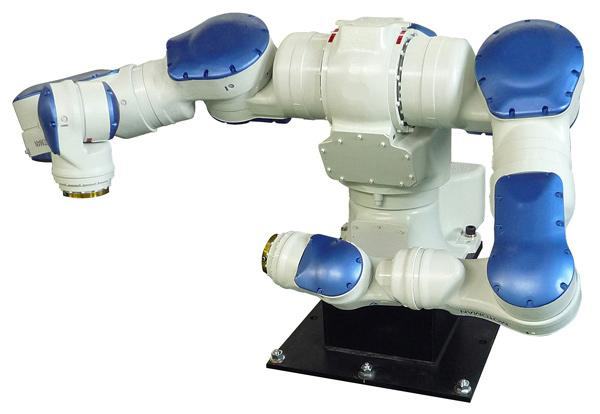
\includegraphics[scale=0.6]{FiguresSoA/TwoArms}\label{dosbrazos}}
\subfigure[Robot Kuka con 6 GDL]{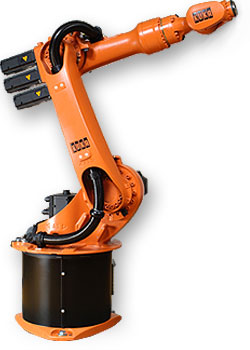
\includegraphics[scale=0.6]{FiguresSoA/KUKA}\label{kuka}}
\caption{Ejemplos de robots industriales}
\end{figure}




%The Motoman SDA5D assembly robot provides "human-like" flexibility in assembly applications. The Motoman SDA-5D DX100has two arms, 7 axes per arm, and one axis for base rotation. The arms can work together to double their payload capacity to 10kg (5kg per arm), which is the lowest payload in the SDA series, or they can work separately to accelerate assembly, part transfer, machine tending, packaging, or other handling applications. Cables and hoses are routed internally in the SDA-5D DX 100to reduce wear and simplify programming.


\section{Historia de la Teleoperación}
La teleoperación tal como la conocemos hoy en día tiene sus orígenes en los requerimientos de la industria nuclear \cite{goertz1952fundamentals}. Inicialmente se usaban pinzas de más de medio metro para separar al operador del material radioactivo, pero a medida que el trabajo con este tipo de material se iba haciendo mayor también aumentaba su  peligrosidad. Se emplearon pinzas con accionamiento remoto separando al operador del material mediante barreras de protección. El trabajo era bastante inc\'omodo debido a las restricciones de las pinzas por su paso por las barreras y la visión de la tarea se realizaba a través de espejos.\\


En 1947 en el Argonne National Laboratory de Estados Unidos se iniciaron las primeras investigaciones lideradas por Raymond Goertz, cuya finalidad era el desarrollo de sistemas de telemanipulación que facilitaran la realización de tareas remotas \cite{goertz1961manipulator}. En 1949 concluyó el desarrollo del primer manipulador teleoperado mecánico, llamado M1 \cite{goertz1952fundamentals},\cite{goertz1954mechanical}. \'Este podría ser considerado el antecesor de los sistemas de teleoperación maestro-esclavo existentes hoy en día. En los años posteriores continuaron los desarrollos basados en mejoras al M1, pero no fue sino hasta 1954 cuando Goertz presentó el primer manipulador maestro-esclavo bilateral con accionamientos eléctricos y servocontrolados, llamado E1.\\


A partir de 1956 Pesanti y Cherel comienzan a realizar un desarrollo de un sistema maestro-esclavo mecánico para la Agencia Atómica Francesa (\textsc{Commisariat de l’Energie Atomique}). Ese mismo año se desarroll\'o el sistema teleoperado Mascot, entre un equipo italiano y el \textsc{Argonne National Laboratory}. A finales de los años 50 se comenzó a aplicar esta tecnología al campo de las prótesis humanas y la rehabilitación en general.\\



En la figura \ref{Goertz} se muestra el telemanipulador de Raymond Goertz, fue un pionero en el campo de la robótica. Específicamente en el área de los robots operados a distancia (telepresecia). En 1951 mientras se encontraba trabajando para la comisión de energía atómica en \textsl{Argonne National Laboratory} desarrollo el primer manipulador de tipo maestro-esclavo con el propósito de manipular materiales radioactivos.


\begin{figure}[ht!]
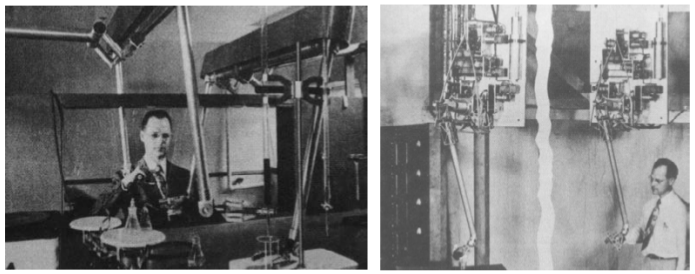
\includegraphics[scale=0.6]{FiguresSoA/Goertz}
\caption{El telemanipulador de Raymond Goertz años 50}
\label{Goertz}
\end{figure}


%La telerob\'otica es una \'area de la rob\'otica que concierne al control a distancia de sistemas rob\'oticos, generalmente a tr\'aves de comunicaci\'on inalambrica por ejemplo  wi-fi,  bluetooth,  radiofrecuencia dependiendo de la distancia o bien por redes de cominicaci\'on cableadas como  Ethernet   




%\begin{figure}
%\centering
%\subfigure[Robot K10 Rover]{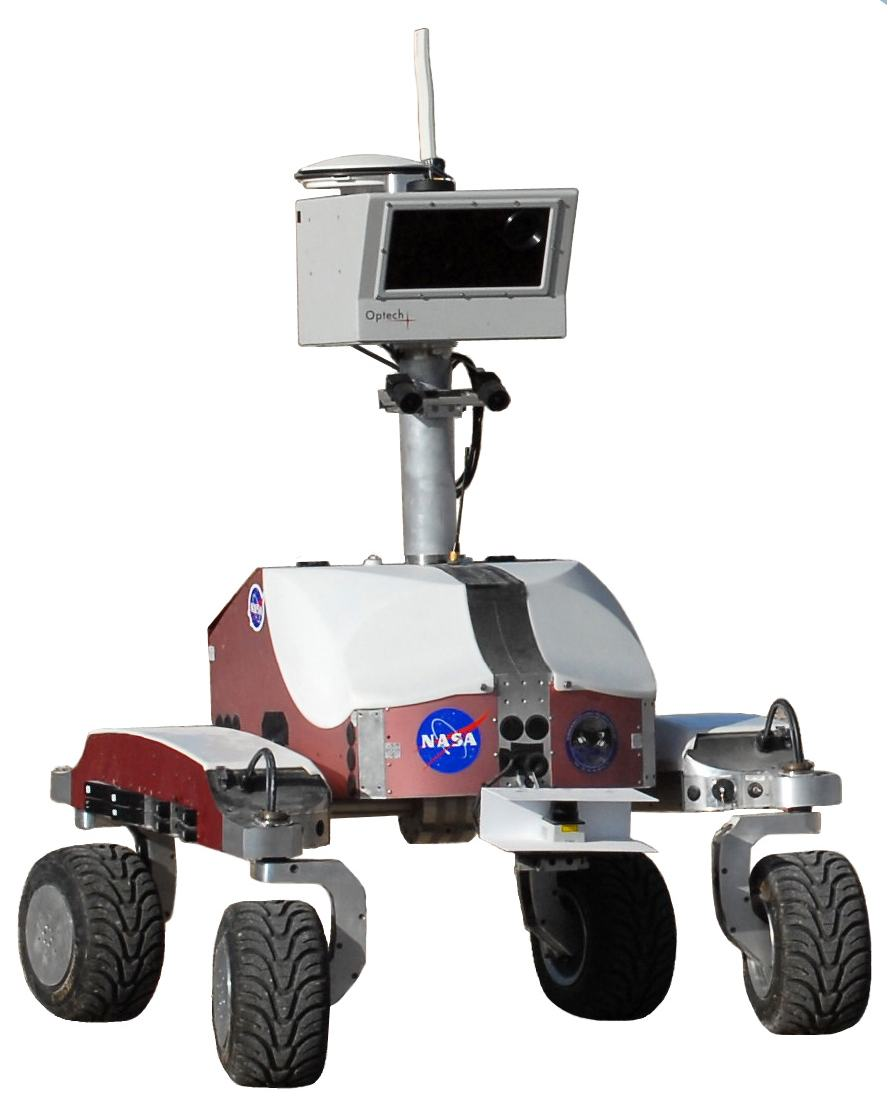
\includegraphics[scale=0.4]{Figures/K10Rover}}
%\subfigure[Retro excavadora controlada a trav{es de un maestro de Kraft Telerobotics]{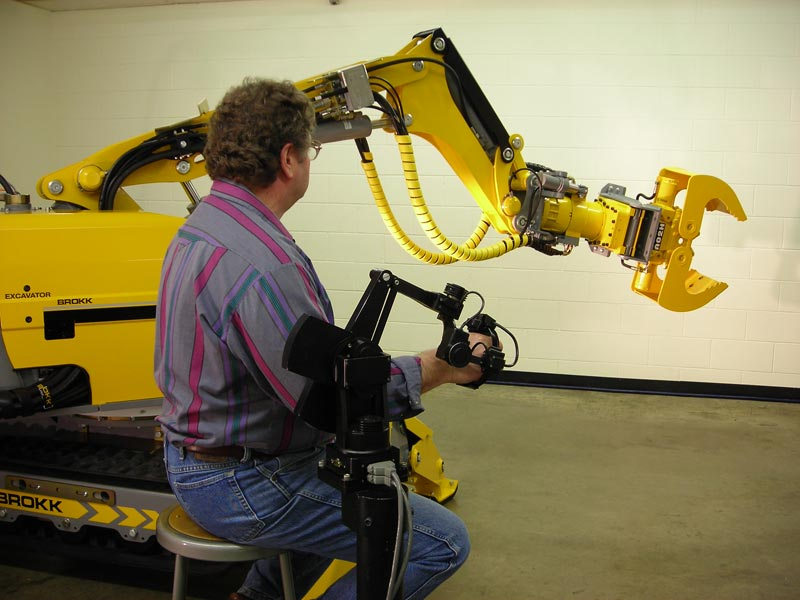
\includegraphics[scale=0.20]{Figures/retroExcavadora}}
%\caption{Ejemplos de robots teleoperados}
%\label{fig:teleoperados}
%\end{figure}




%Telerobotics is the area of robotics concerned with the control of robots from a distance, chiefly using wireless connections (like Wi-Fi, Bluetooth, the Deep Space Network, and similar), "tethered" connections, or the Internet. It is a combination of two major subfields, teleoperation and telepresence.

%Teleoperation

%eleoperation indicates operation of a machine at a distance. It is similar in meaning to the phrase "remote control" but is usually encountered in research, academic and technical environments. It is most commonly associated with robotics and mobile robots but can be applied to a whole range of circumstances in which a device or machine is operated by a person from a distance.[1]

%Teleoperation is standard term in use both in research and technical communities and is by far the most standard term for referring to operation at a distance. This is opposed to "telepresence" that is a less standard term and might refer to a whole range of existence or interaction that include a remote connotation.

%A telemanipulator (or teleoperator) is a device that is controlled remotely by a human operator. If such a device has the ability to perform autonomous work, it is called a telerobot. If the device is completely autonomous, it is called a robot. In simple cases the controlling operator's command actions correspond directly to actions in the device controlled, as for example in a radio controlled model aircraft or a tethered deep submergence vehicle. Where communications delays make direct control impractical (such as a remote planetary rover), or it is desired to reduce operator workload (as in a remotely controlled spy or attack aircraft), the device will not be controlled directly, instead being commanded to follow a specified path. At increasing levels of sophistication the device may operate somewhat independently in matters such as obstacle avoidance, also commonly employed in planetary rovers.

%Devices designed to allow the operator to control a robot at a distance is sometimes called telecheric robotics.

%Two major components of Telerobotics and Telepresence are the visual and control applications. A remote camera provides a visual representation of the view from the robot. Placing the robotic camera in a perspective that allows intuitive control is a recent technique that although based in Science Fiction (Robert A. Heinlein's Waldo 1942) has not been fruitful as the speed, resolution and bandwidth have only recently been adequate to the task of being able to control the robot camera in a meaningful way. Using a head mounted display, the control of the camera can be facilitated by tracking the head as shown in the figure below.

%This only works if the user feels comfortable with the latency of the system, the lag in the response to movements, and the visual representation. Any issues such as, inadequate resolution, latency of the video image, lag in the mechanical and computer processing of the movement and response, and optical distortion due to camera lens and head mounted display lenses, can cause the user 'simulator sickness' that is exacerbated by the lack of vestibular stimulation with visual representation of motion.

%Mismatch between the users motions such as registration errors, lag in movement response due to overfiltering, inadequate resolution for small movements, and slow speed can contribute to these problems.

%The same technology can control the robot, but then the eye–hand coordination issues become even more pervasive through the system, and user tension or frustration can make the system difficult to use.

%Ironically, the tendency to build robots has been to minimize the degrees of freedom because that reduces the control problems. Recent improvements in computers has shifted the emphasis to more degrees of freedom, allowing robotic devices that seem more intelligent and more human in their motions. This also allows more direct teleoperation as the user can control the robot with their own motions.

%Interfaces

%A telerobotic interface can be as simple as a common MMK (monitor-mouse-keyboard) interface. While this is not immersive, it is inexpensive. Telerobotics driven by internet connections are often of this type. A valuable modification to MMK is a joystick, which provides a more intuitive navigation scheme for planar robot movement.

%Dedicated telepresence setups utilize a head mounted display with either single or dual eye display, and an ergonomically matched interface with joystick and related button, slider, trigger controls.

%Future interfaces will merge fully immersive virtual reality interfaces and port real-time video instead of computer-generated images. Another example would be to use an omnidirectional treadmill with an immersive display system so that the robot is driven by the person walking or running. Additional modifications may include merged data displays such as Infrared thermal imaging, real-time threat assessment, or device schematics.




\section{Componentes de un sistema robótico teleoperado}


Una manera sencilla de describir un sistema teleoperado de robots es mediante un operador que envía instrucciones a un robot remoto, el cual ejecutará las órdenes correspondientes y enviará información de su estado y del entorno en el cual se encuentra. Esta información realimentada al operador será la que le permita cerrar el bucle de control del sistema teleoperado. Dentro de este ciclo existen otros elementos que intervienen y que son vitales para el funcionamiento del sistema, por lo que es necesario que sean tratados de manera individual. Para facilitar la identificación de todos los componentes de un sistema teleoperado, se va a hacer una división del sistema de acuerdo a su localización. En la figura , se puede observar que un sistema teleoperado básicamente puede ser dividido en tres partes: entorno local, entorno remoto y canal de comunicaciones.\\


\section*{Entorno Local}
En el entorno local se ubica el operador humano que es el encargado de controlar la ejecución de la tarea remota. Deberá contar con dispositivos de actuación que generen los comandos del operador para ser enviados al robot al entorno remoto. Para que el operador pueda tener conciencia del trabajo que está realizando se necesita dotar a la interfaz del sistema teleoperado de dispositivos de realimentación con los que el operador pueda tener información de la ejecución de la tarea. Dependiendo de la complejidad de la tarea y las condiciones de operación, puede ser necesario cerrar un bucle de control en la zona local, donde se presentan al operador ciertas ayudas que le faciliten la manipulación, bien sea para mejorar su desempeño o para superar adversidades propias a la aplicación como por ejemplo los retardos en la comunicación.




\subsection*{Operador}
El operador es la persona encargada de realizar la tarea y el elemento que cierra el bucle de control. Su intervención puede ser diversa, dependiendo de la aplicación y puede ir desde un control absoluto, pasando por un control compartido hasta otro supervisado.




\subsection*{Dispositivos de actuación}
Son los dispositivos encargados de capturar los comandos generados por el operador para ser transmitidos al manipulador remoto. Existe una gran variedad de dispositivos capaces de realizar esta función, cada uno con características propias, ventajas y desventajas. Entre los más comunes podemos nombrar: teclados, ratones, joysticks, dispositivos maestros, dispositivos maestros con reflexión de fuerza, paletas, pantallas táctiles, pedales, etc. Los joysticks generan habitualmente comandos de velocidad, mientras que los maestros generan comandos de posición, aunque también puede ser programado para generar comandos de velocidad. Es posible hacer uso de otro tipo de dispositivos, simplemente cambiando el medio a través del cual se emiten los comandos, por ejemplo micrófonos para comandos de voz, cámaras para sistemas de captura de movimiento. Un estudio más detallado de los mismos puede ser encontrado en \cite{Ferre2007a}.


\subsection*{Dispositivos de realimentación}
Son los dispositivos encargados de presentarle al operador cualquier tipo de información relacionada con el desarrollo de la tarea que está realizando. Un operador no puede realizar una operación si no puede ver qu\'e es lo que está haciendo. Como en la actualidad prácticamente en todas las aplicaciones teleoperadas el entorno local se encuentra físicamente separad del entorno remoto, el dispositivo de salida indispensable en cualquier operación es el TV o monitor a través del cual se le presentará al operador imágenes de la tarea. Los monitores también son capaces de presentarle al operador información de tipo textual, gráfica o  de imágenes compuestas entre realidad y simulación. Existen maestros y joysticks con reflexión de fuerzas que son capaces de presentarle al operador fuerzas de contacto y manipulación relacionadas con la tarea ejecutada, ademas de cumplir la función de dispositivo de entrada. También es posible hacer uso de altavoces para emitir sonidos, alarmas o información auditiva al operador.


\section*{Entorno remoto}
Es el entorno en el que se encuentra ubicado el robot esclavo y se llevan a cabo la tarea. Es importante resaltar que a diferencia del robot industrial, el entorno de trabajo de un robot usado como manipulador teleoperado, es por lo general, no estructurado, variable o desconocido. Debido a que el operador humano es el que cierra el bucle de control del manipulador esclavo, \'este no requiere de gran precisión en sus movimientos (siempre y cuando el error no sea acumulativo) ya que el operador realizará las correcciones necesarias.



\section*{Canal de comunicaciones}
A través del canal de comunicaciones fluye la información desde el entorno remoto hacia el entorno local y viceversa. Pueden usarse distintos métodos o distintos dispositivos como canal de comunicaciones, la transmisión de información puede llevarse a cabo por medio de cables o sin ellos, las características principales para elegir un canal de comunicaciones suelen ser el ancho de banda, retardos temporales y la robustez de los protocolos de comunicación. Algunos ejemplos pueden ser Internet, redes de fibra óptica, comunicación Serie RS-232, USB, radio frecuencia, entre otras, aunque también depende de la distancia que se tenga entre el entorno remoto y el entorno local. Por un lado el ancho de banda se refiere a la cantidad de información que el canal es capaz de transmitir, mientras que el retardo temporal lo determina el tiempo que tarda la información en ir desde una zona a la otra.


 

%\section*{Modelado de los Elementos del Sistema Robótico Teleoperado}
%Para realizar el estudio de los distintos esquemas, generalmente pueden utilizarse dos métodos de modelado: el método de \textsc{Euler-Lagrange} por medio de la energía del sistema, o bién por el método de \textsc{Newtom-Euler} por medio de las ecuaciones de la cinemática Las ventajas de utilizar el Método de energías de \textsc{Euler-Lagrange} son: que tenemos las ecuaciones resumidas en una forma más compacta involucrando también las matrices de coriolis y la posibilidad de modelar eslabones deformables con su energía de deformación. 


%\section*{Modelado del Operador}
%aquí falta lo del modelado tipo kelvin y todo eso


%\section*{Modelado del Entorno}



%\section*{Algoritmos de Control Bilateral}

%Es la principal área de investigación desde los inicios de la teleoperación, con lo cual es bastante extenso el material referente a este tema. Existen diversos esquemas aplicando control clásico, moderno, teoría de cuadripolos, variables de ondas, etc. No se detallarán esos esquemas porque en la presente tesis existen otros capítulos dedicados a estos temas donde serán tratados con mayor profundidad, simplemente se mencionarán algunos de los desarrollos que diversos investigadores han implementado en la actualidad. Vale la pena resaltar que en lo que a control se refiere un tema que se encuentra en pleno desarrollo es el del control con retardos en las comunicaciones, impulsado inicialmente por su aplicación el sector espacial y submarino, y especialmente motivado en la actualidad por la implementación de sistemas haciendo uso de Internet como medio de comunicación. En el trabajo realizado en [Richard 03], se hace un resumen de los principales modelos usados para describir el retardo temporal, algunos de los esquemas de control usados y problemas abiertos en este campo como por ejemplo: la implementación de los sistemas con retardo temporal de manera digital, identificación adaptativa del retardo, captura y manejo de información relacionada con el retardo, uso de las propiedades estocásticas del retardo. Otro trabajo como el presentado por Blake Hannaford [Hannaford 02], se muestra un método basado en la energía, controlando una interfaz háptica para asegurar un contacto estable bajo una gran variedad de condiciones de operación, como el contacto con entornos de gran rigidez, limitando la fuerza de control y entorno con retardos. Se analiza la estabilidad del sistema en términos de la definición de la pasividad en el dominio del tiempo. Se define el Observador de Pasividad que mide el flujo de energía entrante y saliente de uno o más subsistemas en tiempo real.\\
 


%Un comportamiento activo se verifica con un valor negativo del Observador de Pasividad en cualquier momento. También se define el Controlador Pasivo, un elemento adaptativo disipante, que en cada tiempo de muestreo, absorbe exactamente la salida de energía neta (en caso de haberla) medida por el Observador de Pasividad. Existe un esquema de control bilateral basado en la realimentación hacia adelante (Feedforward) para telemanipuladores lineales dinámicamente parecidos, con escalado cinestésico y de potencia, el mismo se puede encontrar en [Lee 03]. La ley de control propuesta, modela al operador como una herramienta mecánica rígida pasiva con inercia aparente programable parecida al operador humano y al entorno de trabajo remoto, utilizando Feedforward bilateral de fuerza y control con realimentación de posición. La pasividad del sistema de lazo cerrado es robusta ante imprecisiones en las medidas de fuerzas y errores de modelado. La coordinación de errores y aspectos generales de movimiento de la teleoperación son controladas individualmente. El esquema propuesto es aplicable a sistemas generales teleoperados no lineales si se garantiza el uso de una alta ganancia de realimentación. Existen otros trabajos cuyo objetivo es el estudio de ciertas condiciones de funcionamiento como por ejemplo el retardo en las comunicaciones, en este sentido, [Niculescu 02] realiza un análisis de la estabilidad de un esquema de control de teleoperación a lazo cerrado ante la presencia de retardos en la comunicación. Derivando condiciones de estabilidad en el dominio de la frecuencia analíticas y fáciles de verificar. 


%Se estudian casos de independencia del retardo así como intervalos de retardos. La novedad de este trabajo radica en la simplicidad de la caracterización de regiones de estabilidad en términos de los parámetros del sistema. Se presentan tanto interpretaciones físicas como diversos ejemplos. Otra metodología de control que se ha empleado es el control combinado de posición/fuerza de sistemas de telepresencia con reflexión de fuerza y retardos en la comunicación como el desarrollado en [Hirche 03]. Presentando un método de diseño de filtros por igualación de impedancias con optimización en el dominio de la frecuencia con la finalidad de conseguir la pasividad en el Operador/Entorno y transparencia en el sistema de telepresencia controlado en posición/Fuerza. De igual manera en un trabajo presentado en [Leeraphan 02] se muestra una metodología muy similar solo que la igualación de la impedancia se realiza de manera adaptativa con el tiempo. Existen estudios detallados del uso, análisis y diseño de sistemas telemanipulados con variables de onda, los mismos se basan en el concepto de la potencia y la energía, como por ejemplo [Niemeyer 04], donde se presenta una modificación o extensión de la teoría de la pasividad, creando robustez ante retardos temporales arbitrarios. En este estudio se muestra que el uso de las variables de ondas ofrecen diversos beneficios como:

%Robustez ante retardos temporales de varias magnitudes, para retardos nulos el sistema se revierte automáticamente a una configuración de teleoperación clásica. Para retardos pequeños, el sistema se mantiene robusto y estable. La impedancia de la onda, o matriz de impedancia, provee un mecanismo de ajuste on-line, permitiendo al usuario configurarlo para movimientos rápidos, o reflexión de fuerza sensitiva, dependiendo de la tarea. Mediante el uso de las integrales de onda, el sistema puede combinar toda la información relevante, por ejemplo: posición, velocidad, aceleración, fuerza, en una simple cantidad, reduciendo los requerimientos de transmisión. Vale la pena resaltar que aplicando esta filosofía, los autores efectuaron la teleoperación de un robot con un retardo constante de 2 segundos, así como también retardos variables a través de Internet de 50 mSeg a 1 Segundo. Otro trabajo relacionado con el uso de las variables de onda es el presentado en [Munir 02], donde se realiza un estudio usando las variables de ondas, pero en este caso el grueso del desarrollo se centra en la incorporación de un predictor de Smith, un filtro de Kalman y un regulador de energía al esquema con la finalidad de mejorar la estabilidad del sistema. El predictor no necesita conocer las condiciones iniciales, y el filtro de Kalman eventualmente convergerá al estado interno correcto del esclavo visto desde el lado de la comunicación del maestro. Ya que el estado del esclavo se ve afectado directamente por su interacción con el entorno, y el predictor depende del filtro del Kalman para estimar el estado interno del esclavo, no se necesita medir las fuerzas ejercidas por el entorno al maestro. Se muestra que el sistema es estable aún en la presencia de incertidumbre en el modelo del sistema remoto. Otro trabajo relacionado con el uso del predictor de Smith, puede encontrarse en [Ganjefar 03], donde se presenta un estudio del comportamiento de un sistema de teleoperación con errores de modelado y de retardo de comunicación con el uso del predictor\cite{welch1995introduction}.\\
 
 

%Se presenta unas condiciones de estabilidad para el caso de los errores de modelado, que sirve de ayuda a los diseñadores para asegurar la estabilidad del sistema. También se realiza un estudio del efecto de la predicción del retardo en la estabilidad y se demuestra que dicha predicción puede mejorar el desempeño del sistema. Existen otros trabajos cuya finalidad es la de obtener nuevos esquemas, como por ejemplo [Ryu 04], donde se presenta un nuevo esquema de control basado en el concepto de la pasividad, con la finalidad de garantizar la estabilidad de la teleoperación ante una gran variedad de entornos y velocidades de operación. Se ha extendido un método basado en la energía de una red de 1 puerto a una red de 2 puertos, estudiando la implementación de un observador y un controlador de pasividad. El controlador desarrollado no mejora el desempeño (transparencia), sino preserva el desempeño garantizando la estabilidad, para un sistema de gran desempeño, mediante la inclusión de un observador y un controlador de pasividad a un esquema bilateral convencional. Con relación al tema de la transparencia en la teleoperación con retardos en las comunicaciones, en [Zaad 02] se estudia las ventajas de emplear la reflexión de fuerza local, para mejorar la estabilidad y el desempeño. Se presentan 2 esquemas de control de 3 canales, 1) Arquitectura de compensación de fuerzas por el operador y 2) Arquitectura de compensación de fuerzas por el entorno, ambas son perfectamente estables bajo condiciones ideales, y se analiza su estabilidad rigurosamente ante la presencia de retardos. Existen desarrollos de nuevas metodologías de reflexión de fuerzas, como puede observarse en [Love 04], donde se reducen los requerimientos de energía por parte del operador sin sacrificar la estabilidad, el autor explica que la estabilidad en los sistemas de teleoperación con reflexión de fuerzas requiere altos niveles de amortiguamiento, lo que a su vez incrementa los requerimientos de energía por parte del operador. Se realiza una aproximación novedosa de modelado e identificación del entorno remoto, combinando la identificación recursiva convencional de múltiples entradas y múltiples salidas de mínimos cuadrados, identificando en tiempo real la impedancia del entorno con un modelo discretizado del entorno. Esta metodología genera una representación de la dinámica del entorno variante en el tiempo, dependiente de la posición. Seguido a la estimación del entorno, se adapta la impedancia del robot maestro, respecto al modelo dinámico del entorno. Tanto la estimación del entorno como la adaptación de la impedancia se realizan simultáneamente y en tiempo real. Se demuestra prácticamente, mediante experimentación que esta metodología disminuye lo requerimientos de energía por parte del operador, mientras que se provee de suficiente amortiguación para asegurar la estabilidad en el contacto. Otras investigaciones estudian aspectos como por ejemplo, la relación entre los parámetros de impedancia y factor de escalado derivados del uso del concepto de máxima estabilidad y pasividad, como puede encontrarse en [Cho 02]. En la actualidad aún existen investigaciones de interés basadas en los esquemas bilaterales de control clásico, por ejemplo en [Ni 02] donde se desarrolla un esquema de control posición-posición basado en la adaptación de ganancia, con la finalidad de reducir el costo de los sistemas de teleoperación evitando el uso de sensores fuerza/par que ofrece una transparencia pobre. El mismo se basa en la detección de los cambios de impedancia en el lado del esclavo, luego las ganancias de los controladores del maestro y del esclavo son cambiadas en consecuencia. Se presentan resultados experimentales para demostrar la efectividad de este esquema.\\

%Finalmente, en [Benedetti 01] se describe una arquitectura mejorada para el control de la teleoperación con reflexión de fuerzas, en presencia de retardos en las comunicaciones entre maestro y esclavo, está basada en la transformación de variables de onda y la identificación de las propiedades del retardo. Este esquema consigue mejor desempeño en el seguimiento de posición y fuerza que otros esquemas similares, mediante la estimación del valor actual del retardo y compensando sus variaciones ajustando un parámetro de control. También se derivan algunas propiedades analíticas de dicho esquema y demuestra el desempeño del esquema simulando un sistema teleoperado.


\section{Interfaces Hombre-Máquina}
Las interfaces hombre m\'aquina (del ingl\'es \textsc{Human-Machine Interface HMI})de un sistema teleoperado son el puente que une al operador con el entorno de trabajo. Como se mencionó anteriormente, está compuesta por los dispositivos de entrada, dispositivos de salida y el control en zonal local. Debe ser sencilla de manejar, robusta, completa y sobre todo facilitar al operador la realización de las tareas remotas. En \cite{Ferre2007a}, se identifican tres puntos que debe cumplir una interfaz, a saber:

\begin{enumerate}
\item  Establecer todas las conexiones necesarias entre el operador y la zona remota de trabajo. Se dan dos tipos de conexiones: las de actuación del operador sobre el entorno remoto y, en sentido contrario, las de realimentación de información hacia el operador.

\item Facilitar la ejecución de tareas permitiendo al operador enviar comandos de alto nivel referentes al trabajo a realizar, a la vez que posibilite su actuación directa cuando sea preciso.

\item Suministrar al operador toda la información necesaria del entorno de trabajo con el fin de que alcance el mayor grado posible de transparencia. Esto le permitirá ejecutar tareas con destreza, así como facilitarle la supervisión de las tareas semiautomáticas.

\end{enumerate}

Debido a la  función vital que cumple la interfaz dentro del sistema teleoperado, se realizan gran cantidad de desarrollos e investigaciones con la finalidad de aumentar cada día más sus capacidades.\\

% Entre los principales puntos en los cuales se enfocan las investigaciones en la actualidad tenemos:\\


%Estudio del desempeño de las Interfaces: Cuando se desarrolla la interfaz de un sistema teleoperado, para poder llegar a alguna conclusión de su desempeño, no solo se tiene que evaluar por su comportamiento técnico como tal, sino al ser la conexión entre el entorno remoto y el operador, es necesario evaluar también su relación con el operador, ya que aún cuando una interfaz técnicamente sea perfecta si los operadores no pueden manejarla por su complejidad, o porque les sea muy incomoda, no se puede implementar en una aplicación real. Por ello es que se han realizado investigaciones en cuanto a la manera de evaluar el desempeño de las interfaces. Existen numerosos estudios de como determinar lo que denomina Calidad de la Experiencia, que es la relación que mantuvo la interfaz con el operador durante la realización de la tarea.Para estudiar esa relación se proponen 3 métodos de recolección de información:\\


%\begin{enumerate}
%\item Medidas Sujetivas: Se obtienen preguntando directamente al usuario como se siente. Estas preguntas pueden ser mediante cuestionario o entrevista y también se pueden clasificar: a) De hecho: son las preguntas que recogen información
%como la edad, años de experiencia con computadores, nivel de educación. B) Tipo opinión: Se refiere a los pensamientos del interrogando acerca de estímulos externos, otras personas u objetos. C) Preguntas de actitud: Se refieren a las
%respuestas internas del interrogando respecto a eventos y situaciones relacionadas con un producto en particular.
%
%\item Medidas de Desempeño: Son medidas prácticas, menos propensas a errores que los cuestionarios. Las medidas pueden ser la cantidad de errores cometidos, tiempo de ejecución, precisión en las operaciones, etc.
%\item Medidas fisiológicas: Son medidas como el estrés, la actividad cerebral, la cyber-enfermedad.
%\end{enumerate}
%
%Las medidas que pueden reflejar la cyber-enfermedad son: el ritmo cardíaco. Niveles de cortisona en la saliva y estabilidad postural. En ese estudio se concluye que una buena calidad de la experiencia se obtiene maximizando 3 dimensiones:\\
%
%\begin{enumerate}
%\item  El disfrute de la experiencia por el operador.
%\item  Su habilidad de lograr sus objetivos.
%\item  La menor cantidad práctica de estrés e incomodidad.
%\end{enumerate}
%
%A la hora de que un investigador tenga que escoger un instrumento para medir cualquiera de esas dimensiones debe escoger el mejor instrumento, a manera general propone:\\
%
%\begin{enumerate}
%\item  Para el disfrute de la experiencia, como estado interno del usuario, se mide mejor con un instrumento sujetivo, como un cuestionario o entrevista.
%\item El proceso hacia el objetivo, el comportamiento del usuario, generalmente se miden mejor con una observación del comportamiento.
%\item  El estrés, incomodidad, son medidas que se miden con instrumentos fisiológicos.
%\end{enumerate}
%
%Reflexión multisensorial: Debido a la perdida de la información sensorial que ocurre por efectos de la teleoperación, se recurre a lo que se denomina sustitución sensorial, que no es otra cosa que inducir o provocar sensaciones artificiales al operador que estén controladas o generadas mediante la aplicación de las leyes físicas que rigen los movimientos o esfuerzos que se realizan para completar la tarea. Esta sustitución sensorial depende en si de la naturaleza del sentido que se quiera sustituir, por ejemplo: en el caso de la vista, debido a que el operador y el esclavo se encuentran en entornos distintos, se presenta bien sea mediante el uso de un monitor dedicado o una ventana imágenes correspondientes a la tarea que realiza el esclavo. Aparte si se quiere dar la sensación de profundidad que se pierde, se hace uso de técnicas 3D, cámaras estereo. En el caso del oído, bastaría simplemente mediante el uso de micrófonos y parlantes llevar
%al operador los sonidos que se generan en el entorno de trabajo (si la tarea lo requiere). Otra manera es hacer uso de señales sonoras como alarmas o avisos relacionados con la tarea que se esta realizando. Una de las técnicas que más se usa para la sustitución de este sentido es el uso del los maestros con reflexión de fuerza, que no hacen otra cosa que reflejar los esfuerzos que realiza el esclavo en el maestro.\\
%
%En este sentido, en \cite{Ferre2007} se realiza un estudio sobre la reflexión de fuerzas usando métodos gráficos (visual), auditivos (sonidos) y cinestésicos (tacto). Donde se concluye que el uso de la realimentación cinestésica de fuerzas es la mejor forma de presentarle al operador una aproximación de la fuerza ejercida y combinada con una realimentación visual o auditiva realzan la información percibida por el operador, mientras que la combinación de las 3 no mejora la percepción respecto a la obtenida por la combinación de la realimentación cinestésica con la auditiva o visual. En [Williams 02], se hace un estudio de la combinación de la realimentación cinestésica con la visual, donde se muestra una mejora significativa en el desempeño de una tarea, indicada por una reducción de la varianza entre 61\% y 90\% en las fuerzas de contacto, reducción de pares entre 46\% y 92\% usando cualquier medio de reflexión de fuerzas. Y mediante el uso de ambos tipos de reflexión simultáneamente presentaba mejores desempeños.\\
%
%Interfases Multimodales: Este es un tema que ha incrementado su interés entre los investigadores. Una interfaz multimodal es aquella en la cual se le presenta al operador un flujo continuo de información en distintas modalidades de la percepción humana, cinestésica, táctil, visual, auditiva, todo con la finalidad de aumentar el grado de inmersión del operador con la tarea que esta realizando. Muchas de las investigaciones se centran el desarrollo del hardware, en \cite{aleotti2002multimodal} se desarrolla una interfaz multimodal concebida para la teleexploración de entornos remotos, la misma cuenta con realimentación de video, simulador 3D, realimentación vibrotáctil y es manejada usando un guante cybertouch de Inmersion Corp. Inc. En \cite{preusche2002teleoperation}, se desarrolla un sistema de telepresencia multimodal a través de Internet que incluye realimentación visual, auditiva, cinestésica y display predictivo, logrando un gran nivel de inmersión en la manipulación con el entorno remoto.





\subsection{Interfaces Hápticas}
Háptica se refiere al sentido del tacto del mismo modo que óptica se refiere al sentido de la vista o acústica al sentido del oído. De modo que las interfaces hápticas son las que permiten que una computadora se comunique con nosotros a través del tacto, generalmente para darnos una realimentación táctil de alguna interacción. Podemos dividir estas realimentaciones en dos categorías según la información táctil que se pretende replicar: realimentación táctil y realimentación cinestética. La primera proporciona información al usuario a través de las terminaciones nerviosas de la piel dando información sobre textura, geometría o temperatura. La segunda ofrece información sobre la posición y movimiento de la mano, de modo que se obtenga una información de las fuerzas que se están ejerciendo (o del peso de un objeto si se está sujetando) y de la elasticidad o rigidez de lo que se está tocando. Es común hablar de realimentación de fuerza para describir la realimentación táctil y/o la realimentación cinestética.

Las interfaces hápticas permiten simular interacciones con objetos reales, que pueden ser útiles para telepresencia  o teleoperación, sintiendo de ese modo a distancia las fuerzas que se están ejerciendo sobre un objeto, pudiendo por ejemplo sentir la presencia de otra persona tocando un objeto a distancia o teleoperar varios aviones no tripulados \cite{troy2011systems,stigter2007design}. También se utilizan para experimentar la interacción con objetos virtuales, algo muy útil para el entrenamiento, existiendo por ejemplo investigaciones que han terminado como tecnologías comerciales para la capacitación en cirugía \cite{sun}. La tecnología háptica, con un nivel de realismo todavía muy limitado, también está presente en la industria del videojuego.

Existen muy diversas tecnologías y prototipos para la implementación de interfaces hápticas. El desarrollo de estas tecnologías permitirá en combinación con otras tecnologías la implementación de interfaces más naturales, como por ejemplo pantallas táctiles que proporcionen realimentación háptica  de modo que se pueda interactuar con un teclado virtual de forma parecida a  un teclado físico, es decir, sin mirar constantemente el mismo.


Las primeras interfaces hápticas fueron desarrolladas  para el control de servo-mecanismos en grandes aviones con la intención de operarlos a distancia. Estos primeros sistemas  operaban en una única vía de tal forma que la fuerza aplicada en la palanca de control se multiplicaba en las superficies de control aerodinámico (alerones, motores, turbinas, entre otras), pero el piloto no tenía una percepción de la fuerza que estaba siendo aplicada realmente \cite{abel2010pilot,abel2007pilot}. En los inicios de la aviación los pilotos de aviones pequeños sin servo-mecanismos tenían todas las sensaciones acerca de la resistencia del aire en los alerones esto suponía una seguridad en ciertas situaciones de peligro. Con la aparición de los primeros servos, el piloto no obtenía esta sensación. Para resolver este problema se instaló un sistema de control que proporcionaba una resistencia a la  palanca del piloto proporcional al ángulo de ataque de los alerones \cite{troy2011systems,stigter2007design,hanlon2011active}.\\


Por otro lado, los teleoperadores y simuladores que controlaban máquinas y herramientas a distancia  en los cuales el usuario era capaz de sentir las fuerzas aplicadas establecieron un precedente en la investigación de interfaces hápticas. A esto se le denominó teleoperación háptica. Despues del primer  teleoperador háptico desarrollado Goertz en 1950 \cite{goertz1961manipulator,goertz1954electrical,goertz1954mechanical,goertz1952fundamentals}. La realimentaci\'on en fuerza ha sido empleada en muchos tipos de teleoperación como en la exploración de las profundidades marinas \cite{domingues2012human}.\\



Los simuladores hápticos se usan en la actualidad para el entrenamiento de los estudiantes de medicina que pueden ser futuros cirujanos, evitando la necesidad de practicar con pacientes reales \cite{sun,waldron}. También son muy usuales los simuladores de vuelo  para el entrenamiento de los pilotos, los cuales son indispensables hoy en día, ya que gracias a estos se evitan catástrofes aéreas, ayudando a los jóvenes pilotos a obtener experiencia sin necesidad de poner en riesgo sus vidas y reduciendo los costes de este entrenamiento \cite{lam1983flight}.\\ 


A partir de la Primera Guerra Mundial fueron desarrollados  vehículos aéreos no tripulados UAV por sus siglas en inglés (\textsl{Unmanned Aerial Vehicle}), también conocidos por sus siglas en español como VANT, dotados de un sistema de control con realimentacion háptica en los controles de vuelo. Estas aeronaves son usualmente preferidas para tareas que resultan peligrosas para los aviones tripulados \cite{chandler2000uav}. Aunque actualmente estas aeronaves son operadas de forma totalmente autónoma pues el piloto u operador únicamente tiene que fijar las coordenadas de destino en el mapa y el sistema de control de vuelo se encarga de dirigir la aeronave a su destino. En este caso la única tarea del piloto es manejar las cámaras de largo alcance para poder enfocar el objetivo, ya sea para cuestiones de espionaje, seguridad, o marcar las coordenadas donde debe de impactar una bomba o un misil. Es importante destacar que el operador puede tomar control manual sobre la aeronave en caso de emergencia \cite{nikolos2003evolutionary}.\\



La realimentación háptica es comúnmente usada en vídeo juegos. En 1976 el juego de motocicletas \textsl{Moto-Cross}  también conocido como \textsl{Fonz} desarrollado por la compañía \textsl{Sega\textregistered}, fue el primer juego en proporcionar una realimentación de fuerza, la cual se manifestaba al momento de una colisión mediante la vibración de un volante de motocicleta ubicado en la parte superior de la consola \cite{wolf2008video}. Dispositivos hápticos simples usados en la mayoría de los vídeojuegos actuales pueden ser controles, joysticks y volantes de automóvil, los cuales permiten al usuario una realimentación por medio de vibraciones.  La forma más sencilla de proporcionar una sensación háptica en un juego es la vibración en los controles, con la que el usuario puede experimentar algunas irregularidades tales como golpes en un juego de peleas, disparos en un juego de combate o un choque en un juego de carreras de autos \cite{chang2002haptics}.\\



\begin{figure}[htb!]
\centering
\subfigure[Two Phantoms]{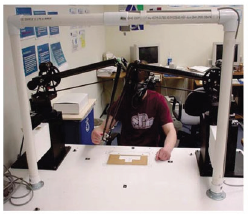
\includegraphics[scale=0.90]  {FiguresSoA/TwoPhamtoms}\label{fig:twophamtoms}}
\subfigure[Cyber Grasp ]{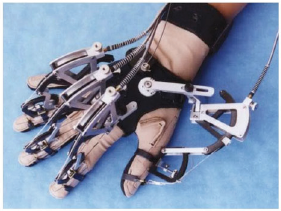
\includegraphics[scale=0.90]{FiguresSoA/CyberGrasp}\label{fig:cybergrasp}}
\subfigure[Spydar]{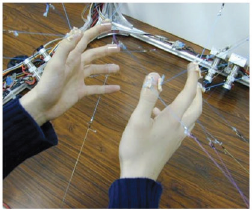
\includegraphics[scale=0.90]{FiguresSoA/Spydar}\label{fig:spydar}}
\subfigure[Hiro III]{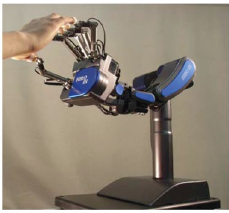
\includegraphics[scale=0.90]{FiguresSoA/hiro3}\label{fig:hiro3}}
%\label{fig1}
\caption{Ejemplo de algunas interfaces hápticas}
\end{figure}

%\cite{Kawasaki,endo2008fpga,endo2011multi,kawasaki2003control,kawasaki2006haptic,kawasaki2007design}
Ejemplos de dispositivos hápticos más parecidas al trabajo que se pretende realizar son: Two Phantoms, CyberGrasp, Spydar y HiroIII, Ver figura 1.  Las interfaces hápticas multidedo antes mencionadas están basadas en el uso de varios dispositivos hápticos de un solo dedo. Algunas toman lecturas de la  posición de la mano humana, para poder aplicar una fuerza en una mano robótica humanoide y tomando datos de sensores en la mano robótica, permitiendo la interacción bidireccional. Otras utilizan la información de la mano humana para producir una interacción con un entorno virtual.\\

 Uno de los dispositivos hápticos de un solo dedo más populares es Phantom de SensAble Tecnologies ver figura \ref{fig:twophamtoms}. \'Este ofrece una solución simple que se basa en una alta precisión en el efector final, mediante la fijación de un punto en el espacio de trabajo por cada dedo. El problema principal de esta configuración radica en las colisiones entre los eslabones del dispositivo que se traduce en una disminución del área de trabajo.\\


Por otro lado han sido desarrollados dispositivos que incluyen varios puntos de contacto y además pueden ser utilizados en varias aplicaciones para ofrecer una mayor destreza de manipulación. Estas soluciones ofrecen un mejor rendimiento en cuanto manipulación y un aumento significativo en el área de trabajo.\\ 

La figura \ref{fig:cybergrasp} muestra el prototipo CyberGrasp que consta de un exoesqueleto que permite el control individual de cada uno de los cinco dedos. Este dispositivo únicamente puede reflejar fuerzas normales en las puntas de los dedos, sin ninguna componente tangencial, y por lo tanto el usuario puede penetrar un objeto tangencialmente sin ninguna realimentación de fuerza. Con este dispositivo es necesario un punto de referencia fijo en la muñeca para poder calcular su localización 3D.\\

 La figura \ref{fig:spydar} muestra un dispositivo háptico basado en una estructura paralela de cables llamado Spydar \cite{lopez2012mechanical}. La versión actual implementa puntos de contacto para todos los dedos. Como se puede observar este tipo de configuración es más eficiente en cuanto a la precisión pero su espacio de trabajo est\'a restringido para evitar que se enreden los cables. Esto limita en gran medida las tareas cooperativas o que involucran el uso de ambas manos. Por otro lado, soluciones más complejas como el robot háptico Hiro III\cite{Kawasaki,endo2008fpga,endo2011multi,kawasaki2003control,kawasakiforce,kawasaki2007design,mouri2005developments,mouri2006novel} también proveen puntos de contacto en todos los dedos. Sin embargo es demasiado sofisticado y requiere del multiples sensores de fuerza/par (uno por cada dedo), lo cual incrementa su costo significativamente.\\
 
  La figura \ref{fig:hiro3} muestra la configuración especular del robot Hiro III. Como Spydar ésta configuración puede presentar inconvenientes cuando se realizan tareas bimanuales debido al limitado espacio de trabajo disponible. 



\subsection{Interfaces Visuales}

La realimentación visual es de vital importancia en las interfaces de teleoperación, ya que si el operador no puede ver lo que esta haciendo no puede realizar ninguna tarea. Es por esto, que muchas investigaciones realizadas buscan mejorar la calidad de la realimentación visual del operador. La mejora en la calidad de la realimentación estéreo es un punto donde se realizan grandes esfuerzos, porque la percepción de profundidad en teleoperación es vital para el buen desempeño del operador. 

%Por ejemplo, en [Hopf 00], se realiza un diseño de un sistema estereoscópico adaptativo basándose en la aplicación de espejos esféricos y óptica colimada, el mismo presenta un alto grado de telepresencia, además mejora las condiciones de visión del operador, permitiéndole trabajar por tiempos mas prolongados. En el centro de investigación Langley de la NASA, también se han realizado investigaciones al respecto, por ejemplo en [Parrish 95], se mostró que el volumen de profundidad disponible se incrementa con el uso de óptica colimada. En [Runde 00], desarrollan un sistema estereoscópico con paralaje de movimiento para la captura y reproducción de imágenes estereo. En el mismo, no se usan dispositivos como gafas esteros o cascos estereos, ya que consideran que de esa manera la sensación es más natural. En [Mulligan 01], se realiza un estudio del desempeño de los algoritmos de generación de imágenes estereo para la telepresencia. En [Adelstein 00], por otro lado, se estudia los efectos de agregar un grado de libertad, el de roll a las plataformas de cámaras de telepresencia al conocimiento espacial del operador. En [Ferre 03], se presenta el diseño de una cámara estereo novedosa, donde la imagen es insertada directamente en la comunicación VGA entre el ordenador y el monitor, evitando consumir recursos del sistema que pueden ser usados en otras tareas, además de la generación de imágenes estereo también tiene la capacidad de efectuar blending, es decir la superposición de imágenes reales con imágenes simuladas. Otras de las líneas de investigación con el uso de la visión es su aplicación no como medio de realimentación al operador, sino como dispositivo de entrada de los sistemas teleoperados. En [Colombo 01], se realiza un estudio de un sistema de captura y reproducción de posturas del cuerpo humano usando modelos computarizados. En [Maaoui 01], se implementa un sistema de las mismas características pero aplicado a un sistema teleoperado. El desafío en estas aplicaciones radica en el cálculo en tiempo real de la posición del operador y su mano, así como su configuración. Para poder emitir comandos de posición o movimiento de una manera más natural, mediante el uso de gestos con las manos o con el cuerpo entero.



%\subsection{Interfaces Auditivas}
%La voz es la principal manera de comunicación de los seres humano y por lo tanto la más natural. Si bien es cierto que los comandos de voz no son la manera más eficiente para el guiado de un robot [Ferre 97], si constituyen un medio ideal para la emisión de comandos de alto nivel [Marin 02] (dependiendo del grado de automatización disponible) a la zona remota o como herramienta de navegación de lainterfaz. Los comandos de voz son ideales para emitir comandos que impliquen cierto grado de automatización, un ejemplo seria la solicitud de cambio de una herramienta, en el caso de su uso como herramienta de navegación de la interfaz, en [Ferre 97] se explica que sirve como medio para desplazarse a través de los menús de la interfaz, con lo cual evitaría que el operador tenga que usar el ratón o el teclado del ordenador, y estar continuamente intercambiando entre el dispositivo maestro y los periféricos del ordenador. Uno de los principales desafíos técnicos que se enfrenta el procesamiento del lenguaje natural es el tratamiento digital de las señales, tal como se especifica en [Juang 02], donde se hace hincapié en que para lograr que el operador actúe de una manera más natural es necesario la implementación de este tipo de sistemas con tecnología manos libres, es decir que el operador no tenga necesidad de usar ningún tipo de dispositivo para interactuar con la interfaz. Esto hace que se presenten complicaciones en su implementación como lo son el ruido ambiental, la señal acústica es función del entorno, el tipo de micrófono usado en el sistema. Se identifican los siguientes puntos en los cuales es necesario profundizar las investigaciones:\\

%El problema del Ruido: Se considera como ruido todas las señales acústicas percibidas por el micrófono que no sean las de la persona autorizada para hablar. Esto incluye ruido ambiental, sonido de máquinas, conversaciones de fondo, etc. Aparte de estas causas existen otras que deterioran la señal acústica como por ejemplo la saturación, la fluctuación de niveles, etc. Pero el ruido es la más dañina. Por lo que es necesario desarrollar métodos para la cancelación del ruido. Entre los métodos pueden ser nombrados:\\

%Cancelación de ruido: Es una de las primeras ideas, básicamente se fundamenta en el uso de la señal ruidosa que se quiere tratar y otra señal de ruido de referencia. Se usa una versión filtrada del ruido de referencia para cancelar el ruido de la señal que se quiere tratar. Este método es impráctico para sistemas manos libres por cuestiones de disponibilidad del ruido de referencia. Método basado en los estimados en corto tiempo del espectro de potencia: Son considerados de alguna manera efectiva. Superficialmente se basa en la estimación del espectro de potencia de la señal de ruido, capturada durante los periodos de inactividad por parte del operador en cuanto a habla se refiere, luego se sustrae del espectro de potencia de la señal ruidosa que se quiere identificar, se resintetiza la señal aumentada usando la información de la fase ruidosa. El problema de la comunicación duplex. La comunicación duplex es cuando 2 usuarios de dos terminales envían y reciben información simultáneamente, en el caso de la teleoperación de un manipulador remoto, esto tendría sentido solo si en la interfaz se encuentra implementado tanto el sistema de reconocimiento de voz como la emisión de señales, alarmas o avisos de manera usando voz sintética. En este caso las investigaciones se enfocan en el desarrollo de algoritmos de cancelación de eco, en pocas palabras suprimir la información proveniente de las cornetas del sistema. Estos algoritmos trabajan estimando la respuesta impulso de la ruta de retorno del eco, la cual es usada hacer una convolución con la señal proveniente de las cornetas para producir un estimado de la señal de eco para propósitos de cancelación. El principal desafío planteado es la estimación de la respuesta impulso de la ruta de retorno del eco acústico. Se han investigado varios algoritmos con propiedades de convergencia rápida durante los últimos años, se han obtenido progresos en la cancelación de eco adaptativo en el dominio de la frecuencia [Benesty 00], que toma ventaja de la propiedad de una matriz circulante para una aproximación eficiente en el proceso de solución, en [Woudenberg 99] se usa un algoritmo de mínimos cuadrados en bloque, que ha sido implementada con éxito en un sistema de reconocimiento de voz automático.\\


%El problema de la reverberación: Cuando la respuesta impulso del cuarto es larga, causa reverberación que tiene un efecto perjudicial en la percepción. Una aproximación es el procesamiento inverso, que involucra la estimación de la respuesta impulso (larga) de la zona local y el filtrado inverso. Sin embargo, se conoce que la respuesta impulso de la zona local es usualmente de fase no mínima y su correspondiente filtro inverso es por lo tanto inestable. Mas aún, ya que la respuesta impulso es también larga, la complejidad computacional tanto en la estimación como la inversión es prohibitiva. Se han propuesto varias ideas interesantes para la inversión de la respuesta impulso de la zona local. En [Wang 91], se propone el uso de múltiples transductores y análisis multibanda, desde el cual la respuesta impulso de la zona local dentro de cada banda de cada transductor es estimado. Luego es aplicada una lógica de selección para escoger un conjunto, o ser apropiado de esas respuestas impulso parciales para la síntesis final de la señal de reverberancia. En [Wang 97], se investiga un algoritmo de inversiones sucesivas también usando un arreglo multitransductor. Un ejemplo del uso de la tecnología de voz puede encontrarse en [Marin 02], donde se realiza una implementación de un sistema de reconocimiento de voz a través de Internet, la interfaz desarrollada permite controlar un robot usando comandos de alto nivel, como por ejemplo: recoge X objeto, muévete a X posición, etc. Otra característica importante, es la capacidad de cambiar la gramática en tiempo real, es decir, una vez que el sistema está corriendo el controlador remoto envía un listado de los objetos de la escena, el módulo de reconocimiento obtiene esta lista y luego recompila la gramática acordemente. Usando esta metodología, se reduce bastante los errores de reconocimiento de voz. El módulo se entrenó con varios usuarios, mejorando el rendimiento del sistema de un 80\% de éxitos en el reconocimiento al 90\%, consumiendo un tiempo aproximado de 0,2 segundos en aceptar un comando verbal. Para la implementación del modulo de reconocimiento de voz, se usa la SDK de reconocimiento y síntesis de voz de Microsoft.




%\section*{Algunos Sistemas de Teleoperación}
%
%\section{Entornos Virtuales}


\section*{Internet como Canal de Comunicación}
Durante los últimos años, Internet ha revolucionado la forma en que nos comunicamos, por ello su crecimiento ha sido exponencial. Prácticamente es posible conectarse en cualquier lugar del mundo. Por eso los investigadores y desarrolladores de aplicaciones teleoperadas han visto en Internet un medio perfecto para establecer comunicaciones con cualquier parte y a un coste muy económico en comparación con otros medios como lo puede ser vía satélite en un canal dedicado. Pero no todo es perfecto, al igual que todas las tecnologías, Internet para el caso de la teleoperación también tiene sus desventajas, y es allí donde están centrados la mayor parte de los esfuerzos de los investigadores para poder superarlas y lograr que esta tecnología abra un nuevo mercado para la teleoperación. Una de las principales líneas de investigación en la cual se están realizando gran parte de los trabajos es en el retardo temporal variable de la comunicación. Como se sabe al establecer una conexión entre dos equipos vía Internet, la información viaja a través de varios servidores, routers, switchs y cada uno tiene distintos niveles de tráfico dependiendo de la cantidad de personas que estén conectadas en ese momento. Esto hace que el retraso de la información en llegar a su destino sea variable, lo cual es un inconveniente al momento de controlar cualquier telerrobot y mucho más si es un control bilateral. Existen múltiples desarrollos que intentan dar una solución a este problema.%, algunas de ellas son:

%Mediante el desarrollo de esquemas y leyes de control que sean estables ante la presencia de retardos variables en el tiempo y de distintas magnitudes, en el apartado de Control en teleoperación se nombraron varios trabajos que guardan relación con el tema de los retardos temporales, por lo que no se volverán a nombrar en este apartado. Entre las técnicas más utilizadas en la actualidad para aproximarse a este problema se encuentran el uso de los esquemas diseñados a partir del concepto de pasividad, y la codificación mediante variables de ondas, entre otras. En este sentido, en [Mirfakhrai 01] puede encontrarse un estudio de los retardos en las comunicaciones a distintas horas del día y con servidores distintos ubicados en áreas geográficamente distintas, en la misma ciudad, en ciudades distintas, en países distintos y en continentes distintos. Mediante ese estudio obtiene un modelo de los retardos de la comunicación asumiéndolo como una respuesta ruidosa del sistema, el tipo de modelo usado es el Auto Regresivo AR. Dicho modelo es usado como un predictor de futuros valores de los retardos, para ajustar automáticamente una ganancia en el controlador optimizando de esta manera el desempeño del sistema. Existen otras aproximaciones en el modelado de los retardos temporales en las comunicaciones, por ejemplo [Ye 02] realiza un estudio estadístico de series temporales densamente muestreadas del RTT (Round Trip Delay, por sus siglas en ingles), usando métodos lineales y no lineales, valiéndose de herramientas gráficas como el espectro de potencia y autocorrelación, determinando que existe una correlación lineal fuerte entre las series y una correlación no lineal no muy fuerte, con lo cual concluye que es posible realizar predicciones con un paso de antelación (one step ahead prediction) del RTT y usan un algoritmo adaptativo lineal basado en el principio de máxima entropía para realizarlo, una explicación más detallada del mismo se puede conseguir en [Liu 02]. Otros trabajos como [Elhajj 01], consideran que no es posible modelar los retardos usando un modelo estadístico simple y especifico, mencionando que el realizar cualquier predicción o asunción respecto a los mismos resultaría en una limitante. Otra manera de manejar los retardos variables en la comunicación, es la presentada en [Oboe 03], donde se propone el uso de un buffer en la entrada tanto del lado del maestro como del esclavo, el buffer se llena de datos y luego se va alimentando de datos a los respectivos controladores a una frecuencia constante, de tal manera que el retardo se mantenga constante, de esta manera se simplifica el diseño de controladores ya que no se verán afectados por retardos variables sino constantes. Sumado a esto se desarrolla una metodología para el manejo de las comunicaciones que incluye la verificación online de los parámetros de la conexión tales como el ancho de banda y el promedio del retardo en la comunicación, con esta información se determina el tamaño del buffer y la frecuencia de adquisición de las señales para mantener el retardo constante.\\

%La otra problemática a la hora de realizar una teleoperación usando como Internet como medio de comunicación, es la perdida de los paquetes; principalmente cuando existe congestión en la red, aumenta la cantidad de paquetes perdidos, esto es un problema sumamente importante, ya que puede llegar a ocasionar un funcionamiento erróneo del esclavo pudiendo provocar desde el mal funcionamiento, hasta la avería tanto del manipulador esclavo como de los objetos manipulados y el entorno de trabajo. En [Oboe 03], se propone el uso de un predictor, que cuando se produce la perdida de un paquete, la salida de ese predictor es usada en su lugar. Existen otros trabajos como el presentado en [Qihong 03], cuya aproximación es proponer un Observador de Estados Futuros (Forward Time Observer), con realimentación de posición, velocidad y fuerza para asegurar que el sistema sea robusto, asintóticamente estable y transparente. En este caso, el ruido es tratado como una perturbación o parámetro de incertidumbre y el observador de estados es usado para predecir el estado del esclavo. El resultado obtenido es un controlador fácil de realizar y con un tiempo de seguimiento del esclavo respecto al maestro más corto que usando métodos convencionales, su desempeño es bastante bueno, de hecho al final tanto en el maestro como en el esclavo no se necesito calcular la aceleración. Cuando los valores de retardo imposibilitan el uso de una realimentación cinestésica en el maestro, bien sea porque el sistema es inestable o porque no se cuenta con los medios técnicos para llevarla a cabo, se ha recurrido a otra técnica de realimentación de fuerzas, mediante la sustitución sensorial (en [Ferre 97] hay un estudio más completo de lo que es la sustitución sensorial aplicado a la realimentación de fuerza), que no es más que transmitir al operador sensaciones a través de otros sentidos que no los naturales en la percepción de la misma. Existen varios trabajos que hacen uso de esta técnica como por ejemplo [Ferre 04], [Williams 02] y [Liu 01] que denomina esta técnica como SoftHaptics.



%\section*{Arquitecturas Basadas en Técnicas de Computación Distribuidas}
%\section*{Arquitecturas de Control con Lazos Locales}
%\section*{Arquitecturas Multimodales y de Telepresencia}


%El sistema es fácil de engañar, se puede engañar haciendole creer que algo se está moviendo de manera continua, con una velocidad mínima de refresco de entre 25 Hz y 30 Hz, mientras que para poder brindar una realimentación háptica se necesita un frecuencia de refresco de por lo menos 1000 Hz, esta es una sifra que ha sido motivo de gran controversia y algunos autores afirman que dicha cifra puede ser menor, Burdea dice que la velocidad mínima de refresco para un sistema háptico es de 300 Hz, mientras ha demostrado experimentalmente que es necesaria una frecuencia de entre 550 y 600 Hz,  





\section{Aplicaciones de la Telerobótica y Telepresecia}

%\subsection{Aplicaciones Militares Espaciales de la Telerobótica }
%
%\begin{figure}[htb!]
%\centering
%\subfigure[Robot Militar Teleoperado]{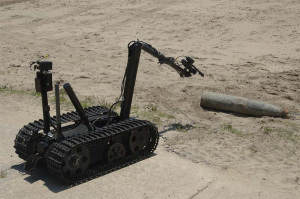
\includegraphics[scale=0.8]{FiguresSoA/militarRobot}\label{fig:robotMilitar}}
%\subfigure[Vehículo aéreo no tripulado]{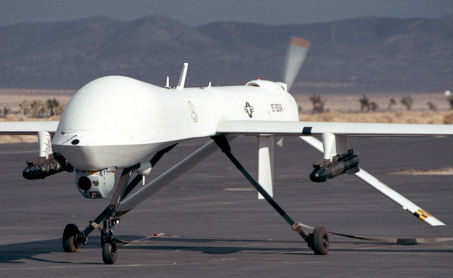
\includegraphics[scale=0.7]{FiguresSoA/drone}\label{fig:drone}}
%\caption{Ejemplos de Robot Teleoperados}
%\end{figure}



%Applications
%Telerobotics for Space
%Soviet telerobotic vehicle Lunokhod-1

%With the exception of the Apollo program most space exploration has been conducted with telerobotic space probes. Most space-based astronomy, for example, has been conducted with telerobotic telescopes. The Russian Lunokhod-1 mission, for example, put a remotely-driver rover on the moon, which was driven in real time (with a 2.5-second lightspeed time delay) by human operators on the ground. Robotic planetary exploration programs use spacecraft that are programmed by humans at ground stations, essentially achieving a long time-delay form of telerobotic operation. Recent noteworthy examples include the Mars exploration rovers (MER) and the Curiosity rover. In the case of the MER mission, the spacecraft and the rover operated on stored programs, with the rover drivers on the ground programming each day's operation. The International Space Station (ISS) uses a two-armed telemanipulator called Dextre. More recently, a humanoid robot Robonaut[2] has been added to the space station for telerobotic experiments.

%NASA has proposed use of highly capable telerobotic systems[3] for future planetary exploration using human exploration from orbit. In a concept for Mars Exploration proposed by Landis, a precursor mission to Mars could be done in which the human vehicle brings a crew to Mars, but remains in orbit rather than landing on the surface, while a highly capable remote robot is operated in real time on the surface.[4] Such a system would go beyond the simple long time delay robotics and move to a regime of virtual telepresence on the planet. One study of this concept, the Human Exploration using Real-time Robotic Operations (HERRO) concept, suggested that such a mission could be used to explore a wide variety of planetary destinations.[5]

%NASA HERRO (Human Exploration using Real-time Robotic Operations) telerobotic exploration concept[5]

%Telepresence/Videoconferencing

%The prevalence of high quality video conferencing using mobile devices, tablets and portable computers has enabled a drastic growth in Telepresence Robots to help give a better sense of remote physical presence for communication and collaboration in the office, home, school, etc. when one cannot be there in person. The robot avatar can move or look around at the command of the remote person.[6]

%There have been two primary approaches that both utilize videoconferencing on a display 1) desktop telepresence robots - typically mount a phone or tablet on a motorized desktop stand to enable the remote person to look around a remote environment by panning and tilting the display or 2) drivable telepresence robots - typically contain a display (integrated or separate phone or tablet) mounted on a roaming base Some examples of desktop telepresence robots include Kubi by Revolve Robotics, Galileo by Motrr, and Swivl. Some examples of roaming telepresence robots include Beam by Suitable Technologies, Double by Double Robotics, RP-Vita by iRobot, Anybots, Vgo, TeleMe by Mantarobot, and Romo by Romotive.

%For over 20 years, telepresence robots, also sometimes referred to as remote-presence devices have been a vision of the tech industry. Until recently, engineers did not have the processors, the miniature microphones, cameras and sensors, or the cheap, fast broadband necessary to support them. But in the last five years, a number of companies have been introducing functional devices. As the value of skilled labor rises, these companies are beginning to see a way to eliminate the barrier of geography between offices.[7] Traditional videoconferencing systems and telepresence rooms generally offer Pan / Tilt / Zoom cameras with far end control. The ability for the remote user to turn the device’s head and look around naturally during a meeting is often seen as the strongest feature of a telepresence robot. For this reason, the developers have emerged in the new category of desktop telepresence robots that concentrate on this strongest feature to create a much lower cost robot. The Desktop Telepresence Robots, also called Head and Neck Robots allow users to look around during a meeting and are small enough to be carried from location to location, eliminating the need for remote navigation.[8]



%\subsection{Aplicaciones Maritimas de la Telerobótica}
%
%%Marine Applications
%
%Los vehículos Marinos Operados Remotamente han sido ampliamente usados para trabajar en aguas profundas o demasiado peligrosas para los buzos.
%
%\begin{figure}
%\centering
%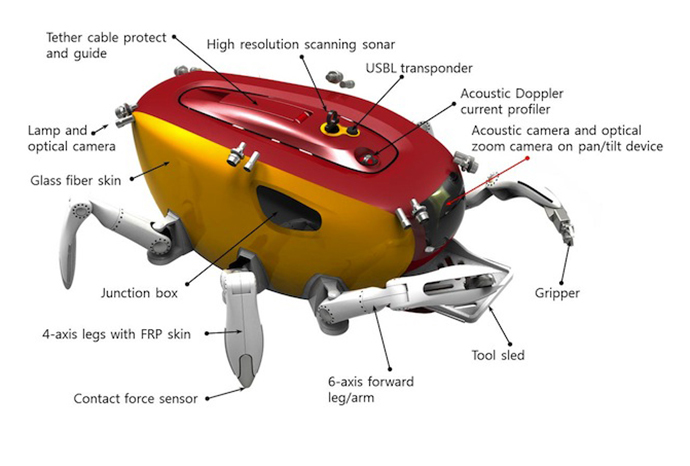
\includegraphics[scale=0.7]{FiguresSoA/crabster}
%\caption{Robot Crabster o CR200 desarrollado por el Instituto Coreano de Tecnología y Ciencias del Oceano }
%\label{fig:cr200}
%\end{figure}
%
%Investigadores del Instituto Coreano de Tecnología y ciencias del Oceano, desarrollaron el robot teleoperado Crabster o CR200 (ver figura \ref{fig:cr200}), diseñado para caminar en el fondo oceánico y soportar las corrientes marítimas, como un crustaceo.\\
%
%El CR200 promete tener todas las posibilidades de ser el robot submarino hexápodo  más grande y ágil del mundo
%
%Las dimensiones del CR200 son de 2.4 m de largo, 2.4 m de ancho y 1.8 metros de alto con sus patas extendidas
%% It’s also way bigger than real crabs: It’s 2.4 meters long, 2.4 meters wide and – when its legs are fully extended – 1.8 meters high.
%
%
%Sus creadores afirman que uno de los mayores retos fue que el CR200 pudiese alcanzar una velocidad de 10 cm/ segundo
%
%los creadores del cr200 esperan que su revolucionario diseño permita hacer construcciones en el fondo del mar. El cr200 puede alcanzar una profundidad de 200 m. y adaptar su postura a diferentes condiciones de presión.


%But it’s also a good deal slower than one of Mother Nature’s crabs, and its creators say that its speed of 10cm/second is one of their main challenges, since it’s difficult to improve Crabster’s stability in strong currents and on rough terrain.



%CR200 hopes to revolutionize the way underwater craft are developed in the future. It can operate down to a depth of 200 meters and adapt its posture to different pressure conditions.

%"We suppose CR200 can conduct seabed mapping, survey and inspection of wrecks, pipelines, ecosystems and pollution down to a 200-meter depth. CR200 will help divers or work instead of them in harsh environments. It also could assist in locating underwater resources, carrying out underwater mining, and responding to oil spill incidents," he said.

%La idea del diseño del cr200 es que pueda hacer un mapeo de las profundidades del mar



%Crabster, designed to scuttle across the ocean floor and survive strong ocean currents and tides just like a real crustacean, has all the chances to be the world’s largest and most agile underwater walking robot, its project team boasts.

%A new crab-like robot is being released into the oceans by the Korean Institute of Ocean Science and Technology.

%CR200, or Crabster as it is affectionately called by its creators, weighs in at over half a ton and has six walking legs, unlike its natural brothers, who have eight. 



%The peculiar design for the robot was chosen as crabs and lobsters can easily control their movements even though they live in stormy waters. Current propeller-driven submersibles do not work properly in fierce tides and human divers are limited to calm, shallow seas.


%It is also kitted out with sonar to scan the seabed for objects of interest, and can send images up to the surface through onboard cameras. 


% Bong Huan jun, the lead researcher of the project, said the robot had performed very well in initial tests but was still undergoing continuous modifications.

%“We are performing tests nearly every day. We upgrade Crabster software for more stable and fast walking and manipulation,” he told CNN.

%The robotic crab will perform its first mission in May, when it will be looking for ancient artifacts in the Yellow Sea where existing craft have been unsuccessful.

%Should this maiden voyage be a success, then Huan jun believes it will have a large worldwide impact.


%He said his team is trying to make Crabster more versatile by trying to program it to swim like a turtle or a diving beetle. They are also considering a hydraulic version for heavy duty underwater work.

%He said he wasn’t sure if the other inhabitants of the deep would know for sure if he is a real crab or not, but said that he hoped that “animals would treat him friendly.” 




%Marine remotely operated vehicles (ROVs) are widely used to work in water too deep or too dangerous for divers. They repair offshore oil platforms and attach cables to sunken ships to hoist them. They are usually attached by a tether to a control center on a surface ship. The wreck of the Titanic was explored by an ROV, as well as by a crew-operated vessel.


\subsection{Telerobótica Médica}


\begin{figure}[htp!]
\centering
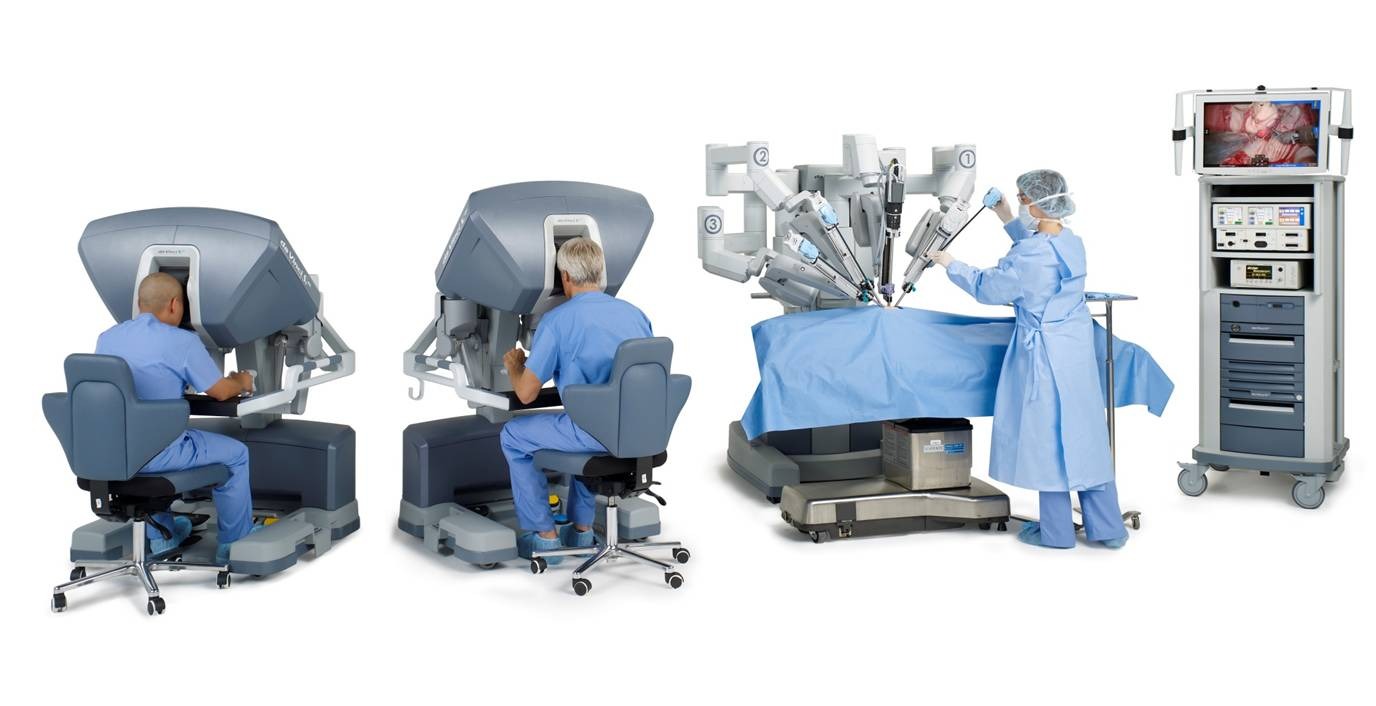
\includegraphics[scale=0.65]{FiguresSoA/News-Da-Vinci-Surgical-Robot-4}
\caption[dos cirujanos ]{Dos cirujanos trabajando de forma cooperativa con el Robot Quirurgico Da Vinci}
\label{fig:davinci1}
\end{figure}


Actualmente se han sido realizadas  grandes esfuerzos e investigaciones en el área de los dispositivos médicos, especialmente para cirugía de mínima invasión. Con los actuales sistemas de cirugía robóticos y de cirugía mínima invasiva los cirujanos son capaces de operar a un paciente a través de un pequeño orificio solo lo suficientemente grande como para permitir la inserción de instrumentos especialmente diseñados, eliminando la necesidad de abrir grandes cavidades que permitiesen trabajar con las manos como se realizaba antiguamente.\\


El Sistema da Vinci es un ejemplo de los últimos desarrollos en el área de la medicina a distancia. El sistema es utilizado para múltiples procedimientos quirúrgicos, especialmente en prostatectomías, es controlado por un cirujano que opera desde una consola y se diseñó para facilitar la cirugía compleja empleando un enfoque mínimamente invasivo. Este factor permite superar las limitaciones propias de la cirugía abierta y laparoscópica, potenciando en términos de visión, precisión y control las habilidades del cirujano. El robot da Vinci no es autónomo,y por ello requiere en todos los casos la intervención y toma de decisiones de un profesional que actúe como operador humano para todas las acciones.\\


El robot quirúrgico Da Vinci se compone de una consola ergonómica desde la que el cirujano opera sentado y que, normalmente, se encuentra en el mismo quirófano. Al lado del paciente se sitúa la torre de visión (formada por controladores, vídeo, audio y proceso de imagen) y el carro quirúrgico que incorpora tres o cuatro brazos robóticos interactivos controlados desde la consola, en el extremo de los cuales se encuentran acopladas las distintas herramientas que el médico necesita para operar, tales como bisturís, tijeras, unipolar, entre otras.\\


El robot da Vinci permite optimizar el rango de acción de la mano humana, reduciendo el posible temblor y perfeccionando todos los movimientos del cirujano. De esta manera, se minimizan las posibilidades de error en relación a otros sistemas quirúrgicos como la laparoscopia, procedimiento en el que el cirujano debe operar de pie con una visión del área anatómica en la que interviene en 2D. En contraposición, el da Vinci ofrece una visión tridimensional de la zona intervenida. Por otro lado, en la laparoscopia, el médico depende de un ayudante para posicionar la cámara correctamente, mientras que en el da Vinci, el cirujano gestiona la cámara de forma totalmente autónoma. También es importante subrayar que el instrumental de la laparoscopia ofrece unos índices de versatilidad limitados mientras que los instrumentos del da Vinci pueden operar de igual forma a cómo lo haría una muñeca humana, lo que permite realizar movimientos altamente precisos en espacios muy reducidos.\\


Otro valor añadido de gran relevancia que ofrece el robot da Vinci al profesional es la posibilidad de poder contar con una visión superior en 3D, alineada entre la zona anatómica afectada y el instrumental, una posición única desde la que se puede trabajar de forma cómoda, intuitiva y precisa.\\


Algunas características del sistema son:
\begin{description}


\item[Consola ergonómica del cirujano]
Es el centro de mando del sistema Da Vinci Si. El cirujano se sienta fuera del campo estéril, en la consola del cirujano, y maneja un endoscopio en 3D y los instrumentos EndoWrist® con los ojos, las manos y los pies mediante dos controladores principales y pedales. El sistema interpreta los movimientos del cirujano y los traduce a escala con movimientos precisos de los instrumentos.

\item[Carro Quirúrgico]
Es el componente quirúrgico del sistema Da Vinci Si, y su función principal es sostener los brazos para instrumentos y el brazo para la cámara. El sistema Da Vinci Si, utiliza la tecnología de centro de control. El centro de control es un punto fijo alrededor del cual se mueven los brazos del carro del paciente. La tecnología de centro de control, permite que el sistema manipule los instrumentos y el endoscopio en la zona de la operación, ejerciendo la mínima presión en la pared del cuerpo del paciente. El usuario del carro del paciente trabaja en el área estéril, ayudando al usuario de la consola del cirujano con el intercambio de instrumentos y endoscopios, y con otras tareas en la zona del paciente. Para garantizar la seguridad del paciente, las acciones del carro del paciente tienen prioridad sobre las acciones de la consola del cirujano.

\item[Torre de Visión]
Aloja el equipo de visualización de procesamiento central del sistema. Posee estantes regulables para incorporar instrumentos quirúrgicos auxiliares opcionales, como unidades electroquirúrgicas (ESU) e insufladores. Durante la operación lo maneja una persona no estéril.


\end{description}



En la figura \ref{fig:davinci1} puede apreciarse  el robot Da Vinci siendo manipulado por dos dispositivos maestros lo cual permite el trabajo colaborativo de ambos, incluso sin la necesidad de estar en el mismo sitio.\\

El robot permite alta precisión de los movimientos ejecutados por el cirujano y el uso de una gran cantidad de instrumentos quirúrgicos distintos de los que cada día se desarrollan más cada día se están desarrollando más instrumentos.\\

La implementación de este sistema permite que los cirujanos puedan trabajar prácticamente desde cualquier parte del mundo.\\


%el robot esclavo Da Vinci cuenta con 4 brazos de 6 grados de libertad cada uno (Ver figura \ref{fig:davinci2}), 

%
%\begin{figure}
%\centering
%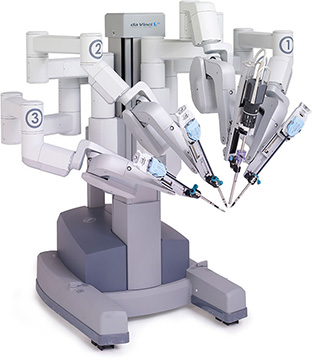
\includegraphics[scale=0.6]{FiguresSoA/davinci-robot}
%\caption{Robot Quirurgico Da Vinci (Esclavo)}
%\label{fig:davinci2}
%\end{figure}

\subsection{Manipuladores Remotos para Entornos Radioactivos}

Los entornos de fusión nuclear están fuertemente restringidos por varios factores, tales como la radiación, altas temperaturas y las dimensiones y pesos de sus componentes. Esto obliga a considerar el diseño de tecnologías de teleoperación como una estrategia viable para realizar tareas en dichas instalaciones.
La fusión nuclear como fuente de energía requerirá el desarrollo de varias tecnologías de teleoperación que pueden ser automáticas o manuales.

Las futuras plantas de energía de fusión similares a la planta de demostración (DEMO) requerirán un sistema de teleoperación excepcional para llevar a cabo actividades de supervisión y mantenimiento. Estas tareas desempeñan un papel fundamental en la gestión global de una planta de energía nuclear.

Las tecnologías de teleoperación se han utilizado con éxito en células de fisión nuclear durante mucho tiempo \cite{Desbats2005} y en el mantenimiento del \textit{tokamak} del \textit{Joint European Torus} (JET) por más de 10 años \cite{Rolfe1999, Rolfe2007} ya que con ello se evitan paradas inesperadas, retrasos de mantenimiento, etc. Además, se ha mejorado la seguridad del personal mediante la reducción de exposición a la radiación y el aumento de la disponibilidad del reactor mediante el uso de equipo reforzado para resistir las condiciones de operación tan cr\'iticas.

En esta sección se presentan los requisitos y características que deben cumplir los sistemas de telerrobótica en un entorno de fusión nuclear. En \cite{Ferre2011,Suarez2011,Queral2011} se presentan estudios completos sobre dichos requisitos y características.

\subsection*{Motivación}
En los últimos años, el establecimiento de la fusión nuclear como fuente de energía requerirá el uso de sistemas teleoperados debido principalmente a la radiación. La industria nuclear ha utilizado los sistemas remotos debido a las restricciones de su entorno desde el principio, pero con los avances tecnológicos se impulsa la implementaci\'on de sistemas cada vez m\'as innovadores.\\

  
Dichos sistemas teleoperados deben hacer frente a: altos niveles de radiación, ultra-vacío, altas temperaturas y el campo magnético toroidal con la intención de realizar la inspección, mantenimiento y reparación de instalaciones de fusión nuclear, tales como el Reactor Termonuclear Experimental Internacional (ITER), DEMO o \textit{International Fusion Materials Irradiation Facility} (IFMIF).

\subsection*{Radiación}
En la tabla~\ref{tab:radiation} se muestran las dosis de radiación para el caso de ITER \cite{ITEROrg.2004}.
\begin{table} [htbp]
\centering
	\caption{Dosis de Radiación para ITER}
	\label{tab:radiation}
	\begin{tabular}{c c c c}
		\hline
		 & \multicolumn{3}{c}{\textbf{Tipo de Inspección}} \\ 
		 																& \textbf{Programada} 	& \textbf{Sin Programar} 		& \textbf{Mantenimiento }\\ 
		\hline
		\multicolumn{1}{l}{\textbf{Tasa de Dosis (Gy/h)$^*$}} 		& $1500$ 							& $15000$ 								& $300$ \\ 
		\multicolumn{1}{l}{\textbf{Duración}} 								& 12 h/semana 					& 12 h/semana 							& 60 h/mes \\ 
		\multicolumn{1}{l}{\textbf{Periodo}}									& $7.5$ años 						& $7.5$ años 								& 32 meses \\ 
		\multicolumn{1}{l}{\textbf{Dosis Total (MGy)}} 	& $2.7$ 								& $27$ 										& $0.6$ \\ 
		\hline
		\multicolumn{4}{l}{$^*$ \small{Datos estimados}}\\
	\end{tabular} 	
\end{table}
El funcionamiento de la electrónica es un problema importante cuando se trata de entornos con radiación\cite{Perrot2004}.
A pesar que varios sistemas de multiplexación no soportan más de 10 kGy, algunos transistores manejan valores nominales de hasta 10MGy.Por lo tanto, es de esperar que sea posible diseñar componentes resistentes hasta 10MGy con estos transistores.El \textit{Radiation Hardness Manual} \cite{Campbell2007} cuenta con un listado de circuitos digitales (flip-flops y compuertas) basados en transistores discretos que resisten dosis en el rango de 10MGy. Por ejemplo, todos los componentes electrónicos del robot PAC \cite{Perrot2004}, descrito en el numeral \ref{robotPAC:sub}, soportan una dosis total de hasta 10 kGy, con una tasa máxima de 10Gy/h.

Todos los materiales estructurales no deben ser susceptibles a la degradación por contaminación.
Componentes sensibles como los sellos deben ser elegidos de acuerdo a su resistencia a la radiación.
Teniendo en cuenta que la única barrera contra la radiación es la masa y que los requisitos dimensionales de los robots no permiten el uso de tales barreras de manera eficaz, todos los componentes a ser utilizados deben probarse para comprobar su funcionamiento bajo altas dosis de radiación.

Se han realizado varios estudios a una amplia gama de componentes con el fin de utilizarlos en la cámara de vacío del reactor, desde fibras ópticas hasta lubricantes, actuadores y cámaras de vídeo \cite{VanUffelen2005, Leroux2006, Bock2008}.Estos estudios muestran que ser\'a posible tener diseños electrónicos compatibles con las limitaciones del entorno de fusión nuclear.

\subsection*{Ultra-Vacío}
Debido a las ultra bajas presiones ($10^{-5} $ Pa) \cite {ITEROrg.2004}, la cámara de vacío (VV - \textit{Vacuum Vessel})  \'esta se debe mantener limpia a toda costa. As\'i, el uso de materiales que liberan gases debe ser evitado. Por lo general, materiales susceptibles a la oxidación y los materiales orgánicos, liberan gases. Por lo que todos los componentes que entran en contacto directo con la cámara de vacío tienen que ser certificados. Una lista de componentes y materiales aptos para ser utilizados en ultra-vacío se puede encontrar en el \textit{ITER Vacuum Handbook} \cite{L.Worth2009}.
El material estructural predeterminado por ITER para estas condiciones es el acero inoxidable 316L (N)-IG \cite{Aiello2011}.

Con el fin de eliminar todas las impurezas y burbujas de gases se realiza el coquizado del robot (normalmente a $240^{o}C $). Generalmente estos puntos que pueden liberar gases se encuentran situados en las imperfecciones de la estructura. El coquizado permite eliminar cualquier rastro de hidrógeno y oxígeno que queda en los poros de los materiales.
Cuando el robot no se puede coquizar en un plazo razonable, lo habitual es confinar en un espacio cerrado las zonas con porosidades.


Existen soluciones de sellado, como la utilizada en el robot AIA \cite{Keller2009}, descrito en la secci\'on \ref{robotAIA:sub}, donde se utiliza Helicoflex\textsuperscript{\textregistered} y sellos de metal.

Por otro lado, se deben utilizar lubricantes no estándar, tales como el disulfuro de molibdeno (MoS$ _ {2} $), carbón tipo diamante (DLC), diseleniuro de tugsteno (WSe$ _ {2} $), sulfuro de tungsteno (WS$ _{2} $) y diseleniuro de molibdeno (MoSe$ _ {2} $) \cite{ogawa2008research}.
En \cite{winer1967molybdenum} se puede encontrar una revisión completa sobre el comportamiento del MoS$ _ {2} $.
Además, el MoS$ _ {2}$ ha sido probado en ultra-vacío y se ha encontrado que ofrece un coeficiente de fricción muy bajo \cite{cizaire2002mechanisms}.
Esta técnica se ha utilizado ampliamente para el diagnóstico de reactores \cite{ogawa2008research}.

\subsection*{Altas Temperaturas}
Para ITER, en la tabla~\ref{tab:temperature} se muestra un resumen de las posibles temperaturas de operación en distintos escenarios \cite{ITEROrg.2004}.

\begin{table} [htbp]
\centering
	\caption{Posibles temperaturas durante inspección para ITER}
	\label{tab:temperature}
	\begin{tabular}{c c}
		
		\textbf{Descripción} 	& \textbf{Temperatura 1\textsuperscript{er} Pared}\\ 
		
		\multicolumn{1}{l}{\textbf{Inspección Programada}} 	& 			$393 K$   \\ 
		\multicolumn{1}{l}{\textbf{Inspección Durante Coquizado}} 	& 		$513 K$   \\ 
		\multicolumn{1}{l}{\textbf{Inspección sin Programar}} 		& 	$393 K$   \\ 
		\multicolumn{1}{l}{\textbf{Mantenimiento}} 					& 	$323 K$   \\ 
		
	\end{tabular} 	
\end{table}

Teniendo en cuenta las altas temperaturas, todas las propiedades de los materiales  (resistencia a la tracción, módulo de elasticidad, etc.) deben ser consideradas a $393 K$ pero el material también debe ser coquizado ($513 K$). Por ejemplo, la mayoría de las aleaciones de aluminio están prohibidas para fines estructurales, ya que debido a sus propiedades mecánicas no son adecuadas para estas temperaturas. Las experiencias con el brazo articulado de Inspección (AIA) \cite{Keller2009} y el sistema de diagnóstico \cite{Smick2005}, dicen que la lubricación puede ser un problema grave también.

\subsubsection*{Distribución de la Temperatura}
Si las diferentes partes del robot están a diferentes temperaturas, puede producirse un problema debido a la dilatación térmica, lo que puede resultar en grietas o estrés adicional en los materiales.

Una solución para evitar este problema consiste en diseñar el robot para alcanzar uniformemente $393 K $. En este caso, las partes exteriores del robot deben actuar como cuerpos negros, con el fin de calentar la totalidad del robot a esa temperatura.

También se deben elegir los materiales con constantes de dilatación cercanas. Para los materiales con constante de dilatación diferente es necesario tener especial cuidado durante la fase de diseño del robot, ya que todas las piezas serán fabricadas a temperatura ambiente ($293 K $  aprox.). Esto también puede ser un problema si la fase de pruebas tiene que hacerse a temperatura ambiente.

\subsubsection*{Aislamiento Térmico}
A pesar de los esfuerzos que se pueden hacer para encontrar componentes compatibles con las altas temperaturas, siempre habrán algunos componentes que no las soporten. En estos casos, la solución es confinar estos componentes en una jaula hecha de material reflectante y puesto que los robots estarán en un ambiente de ultra-vacío, el modo de transferencia de calor principal será la radiación y dicha jaula reflectante tardaría una gran cantidad de tiempo para obtener la temperatura nominal.\\


Por lo tanto un buen diseño implica que dichos componentes puedan estar trabajando durante un largo período de tiempo.\\


Las articulaciones del robot deben ser diseñadas teniendo en cuenta el aislamiento térmico con el fin de minimizar la transferencia de calor por conducción. Esta solución es exactamente la opuesta a la estrategia de distribución de la temperatura. Dado el caso en que estas dos soluciones deban ser utilizadas en un mismo robot, es recomendable trabajar con un modelo muy preciso para cada uno de los casos.

Es evidente que la obtención de un modelo es una dificultad real, ya que la distribuci\'on de temperaturas puede llegar a ser tan compleja como el diseño del montaje. Otro posible solución es diseñar un sistema enfriador con un fluido o gas frío y utilizar un intercambiador de calor fuera de la cámara de vacío.

\subsection*{Campo Magnético}
Un campo magnético tan elevado (3,3 | 6.5MAm $^ {-1} $ / 41000 | 82000Oe densidad de flujo magnético es 4,1 | 8.2T en el vacío) \cite{Izard2009}, en un gran volumen es una situación muy rara, que sólo se encuentra en el mundo de fusión. Incluso la intención de operar bajo estas condiciones un equipo  remoto es única. De hecho, sólo recientemente gracias a los imanes superconductores  es posible generar campos magnéticos sostenidos tan altos \cite{Kiyoshi2006}.\\


Los imanes de cobre pueden producir campos muy elevados (el récord actual es de 100T), pero en un período de tiempo muy limitado \cite{Kiyoshi2006}, por lo que el robot esperaría a que el pulso acabase para realizar las tareas. Hasta ahora, no se habían combinado más restricciones a la del campo magnético, tales como la radiación, altas temperaturas y ultra-vacío en el caso de la fusión nuclear. Sin embargo, los robots que operan bajo la influencia de campos magnéticos elevados no son una novedad, ya que investigadores de la Universidad Johns Hopkins han presentado un sistema robótico completamente compatible con la resonancia magnética \cite{Muntener2006}.\\


En lo que respecta al uso de componentes, aquellos que funcionan utilizando un campo magnético (bobinas de inductancia, transformadores con núcleos de hierro, etc) se verán saturados y serán afectados por fuerzas muy altas, con lo cual, deben ser sustituidos por dispositivos tolerantes al campo magnético como bobinas de aire y transformadores de cerámica \cite{izard2010hardening} .\\


La diferencia principal de una aplicación de fusión nuclear con cualquier máquina superconductora, en general, es que la máquina no está funcionando en el momento del mantenimiento o la inspección, por lo tanto, la perturbación del campo local se puede tolerar, con lo cual los dispositivos electrónicos y los sistemas electromecánicos están permitidos. Los efectos del campo magnético son descritos por las ecuaciones de Maxwell. El desarrollo de las ecuaciones de Maxwell conduce a la fuerza de Lorentz $\mathbf{F}_ {L} $. Cuando no hay ningún campo eléctrico, está escrito como,

\begin{equation}
	\label{ecu:lorentz1}
	\mathbf{F}_{L}=q\cdot{}\mathbf{v}\times{}\mathbf{B}
\end{equation}
En una carga $q$ que se mueve a una velocidad $\mathbf{v}$, ó,
\begin{equation}
	\label{ecu:lorentz2}
	F_{L}=i\cdot{}l\cdot{}\mathbf{u}\times{}\mathbf{B}
\end{equation}

En un conductor con una longitud $l$ y corriente $i$ a lo largo del vector $\mathbf{u}$. $\mathbf{B}$ es la densidad de flujo magnético local en ambas ecuaciones. La ecuación de la fuerza de Lorentz puede ser desarrollada con el fin de demostrar que un campo magnético elevado y constante puede producir un par elevado pero ninguna fuerza: un alto gradiente es necesario para generar una fuerza elevada en un volumen reducido \cite{Izard2009}.

\subsection*{Desarrollos Actuales}
Hoy en día aún no existe ningún robot capaz de soportar las condiciones impuestas por los entornos de fusión nuclear.
Los únicos sistemas que cumplen dichas restricciones son los de diagnóstico, pero deben operar incluso durante la fase de plasma y en muchas ocasiones no se pueden recuperar. Además, el diseño de estos sistemas los hace muy robustos y lejos de poder ser considerados como un robot completo. El sistema de visión \textit{In-Vessel Viewing System} (IVVS) \cite{Neri2007,Neri2009} desarrollado por la ENEA es un ejemplo de los mencionados sistemas de diagnóstico y de lo que se puede hacer con las condiciones dadas.

Dado que estos sistemas de diagnóstico no proporcionan la destreza necesaria para el funcionamiento en la cámara de vacío, la segunda parte de esta sección se centrará en los dispositivos que cumplen algunas de las restricciones, pero con niveles de destreza altos.

\subsection*{Sistema de Diagnóstico}
En fusión nuclear, el entorno de diagnóstico es aún más difícil que el entorno de inspección y mantenimiento, ya que además del ultra-vacío, el sistema de diagnóstico tiene que lidiar con enormes dosis de radiación y altas temperaturas. Además, se utilizan durante la operación del plasma y tienen que hacer frente a las corrientes parásitas (\textit{Eddy currents}) generadas a lo largo de su estructura en caso de un enfriamiento rápido \cite{Izard2009}.

Por estas razones, los sistemas de diagnóstico son muy robustos, sencillos y con capacidades de movimiento mínimas con el fin de evitar fallas. La regla general es el uso de actuadores neumáticos que generen un movimiento lineal. Otros sistemas como mecanismos accionados por temperatura y diseños que utilizan el campo magnético local para generar movimiento también se han utilizado en \textit{tokamaks} anteriores \cite{Smick2005} y esta prevista su utilización en ITER. En este entorno, parece que un gran porcentaje de la carga sobre los actuadores es debido a las corrientes parásitas generadas en las partes móviles \cite{Izard2009}.

%\subsection*{Sonda IVVS}
%El objetivo de la sonda IVVS (\textit{In-Vessel Viewing System}), figura~\ref{fig:IVVS}, para ITER es la medición y visión en la cámara de vacío en condiciones de inspección. En el prototipo construido por la Asociación Italiana de Fusión ENEA \cite{Perrot2004, Neri2007,Neri2009}, un láser se dirige hacia la cabeza de la sonda usando fibra óptica endurecida y luego hacia la pared en inspección utilizando un prisma cuya posición es ajustada por un accionamiento de dos grados libertad.
%
%\begin{figure}[htbp]
%   \centering
%   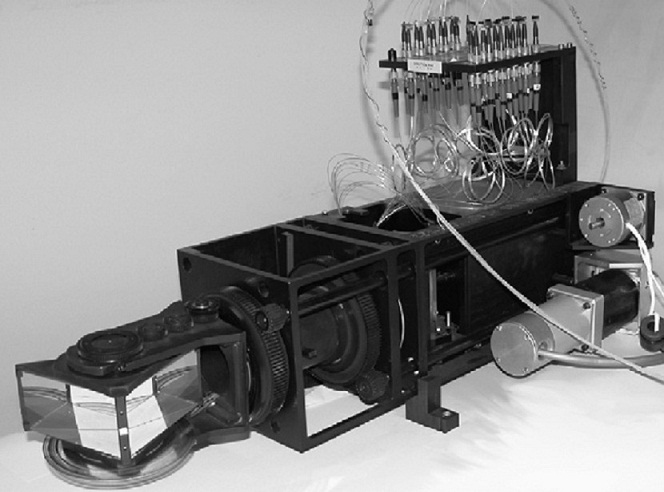
\includegraphics[width=0.5\textwidth]{FiguresSoA/IVVS}
%   \caption{Sonda IVVS}
%   \label{fig:IVVS} 
%\end{figure}
%
%En su último diseño, la sonda es de acero inoxidable AISI 304, pesa 22 Kg., tiene motores ultrasónicos y reductoras para mover el prisma. El marco del espejo es en aleación de titanio para reducir la fricción por las corrientes parásitas, ya que se supone que se mueva a 1 rps \cite{Izard2009}; Las reductoras también son de acero inoxidable AISI 304, con nitruro de titanio para su lubricación.

\subsection*{Brazo Articulado de Inspección AIA}		\label{robotAIA:sub}
El brazo articulado de Inspección AIA \cite{Gargiulo2008,Keller2009,Gargiulo2009, Houry2010}, que se muestra en la figura \ref{fig:AIA}, desarrollado en conjunto por CEA List y los laboratorios IRFM, es una demostración de cómo un brazo articulado de largo alcance puede ser un solución factible para la inspección en la cámara de vacío. Este robot ha sido diseñado para funcionar en ultra-vacío ($10^{-5}$ Pa) y a una temperatura de $120^{\circ}C$ (previamente coquizado a $200^{\circ}C$). Es un brazo de cinco módulos con una capacidad de carga de 10 Kg, con una longitud total de $7,4$ m y 160 mm de diámetro. Su peso total es de 130 Kg.

\begin{figure}[htbp]
   \centering
   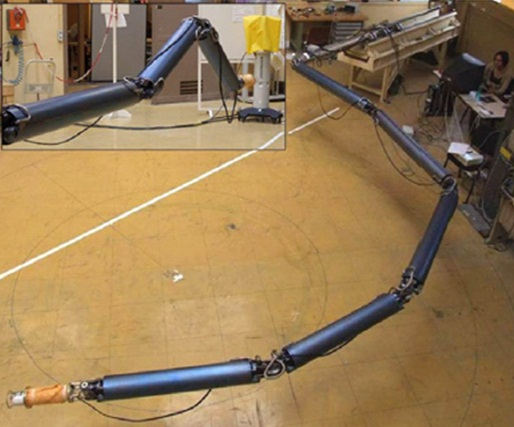
\includegraphics[width=0.6\textwidth]{FiguresSoA/AIA}
   \caption{Brazo Articulado de Inspección AIA}
   \label{fig:AIA} 
\end{figure}

La primera introducción del AIA en el reactor \textit{Tore Supra} en condiciones de operación tanto de ultra-vacío y temperatura se produjo en septiembre de 2008 \cite{Keller2009}.
Se equipó con una sonda de visión endurecida que le permitía observar la erosión de los casquetes limitadores y el funcionamiento de las persianas de diagnóstico.
Además cuenta con una amplia gama de efectores finales desde un láser para la eliminación de tritio hasta tareas ligeras de contacto y calibración de diagnóstico con herramientas de sujeción.
La operación del plasma se reanudó 15 horas después de retirar el robot que es el tiempo necesario para alimentar las bobinas superconductoras \cite{Gargiulo2009}.

La información se transfiere a los módulos gracias a los sistemas de multiplexación.
Cada módulo está equipado con una electrónica de multiplexación \textit{Neurobot} endurecida para las altas temperaturas. También está equipado con un sistema de amplificación para los motores.
Los componentes que no son compatibles con el ultra-vacío están encerrados en cajas anti-fugas de acero inoxidable.

\subsection*{Robot PAC}
\label{robotPAC:sub}
El robot PAC (\textit{The Porteur Articulé en Cellule}) \cite{Perrot2004} mostrado en la figura~\ref{fig:PAC}, es un brazo articulado de 6 metros de largo con una capacidad de carga de 1 Kg y un diámetro exterior de 100 mm.
Se ha desarrollado para aplicaciones de AREVA-NC por CEA LIST y ha sido diseñado para realizar tareas de inspección en celdas calientes. Dichas celdas se encuentran bajo condiciones atmosféricas y de temperatura normales, pero los niveles de radiación son altos, por lo tanto, el robot tiene que resistir una dosis total de 10 kGy.

\begin{figure}[htbp] 
   \centering
   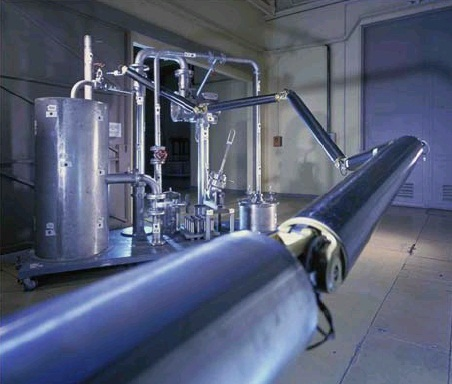
\includegraphics[width=0.6\textwidth]{FiguresSoA/PAC}
   \caption{Robot PAC en una celda caliente de AREVA.}
   \label{fig:PAC} 
\end{figure}

La principal característica demandada a este robot es la movilidad, ya que la celda caliente tiene tuberías complejas.
Es por eso que el robot tiene la misma arquitectura modular con el mecanismo paralelogramo vertical como el AIA en el cual se inspira. La diferencia es que en este caso el mecanismo de paralelogramo compensa la gravedad con un resorte de fibra de vidrio.

\subsection*{Manipulador WHMAN}
El manipulador WHMAN (\textit{Water Hydraulic MANipulator}) \cite{Nieminen2009} es un robot teleoperado con reflexión de fuerzas. Se caracteriza porque es hidráulico y como fluido utiliza agua. El brazo esta equipado con siete articulaciones actuadas que le permiten contar con seis grados de libertad. El diseño actual pesa 185 kg y sus materiales base son aleaciones de aluminio y acero inoxidable. Funciona con una presión de linea de 210 bar y requiere un caudal de 10 lpm. Además requiere una linea neumática a 6 bar y una conexión eléctrica.

\begin{figure}[htbp] 
   \centering
   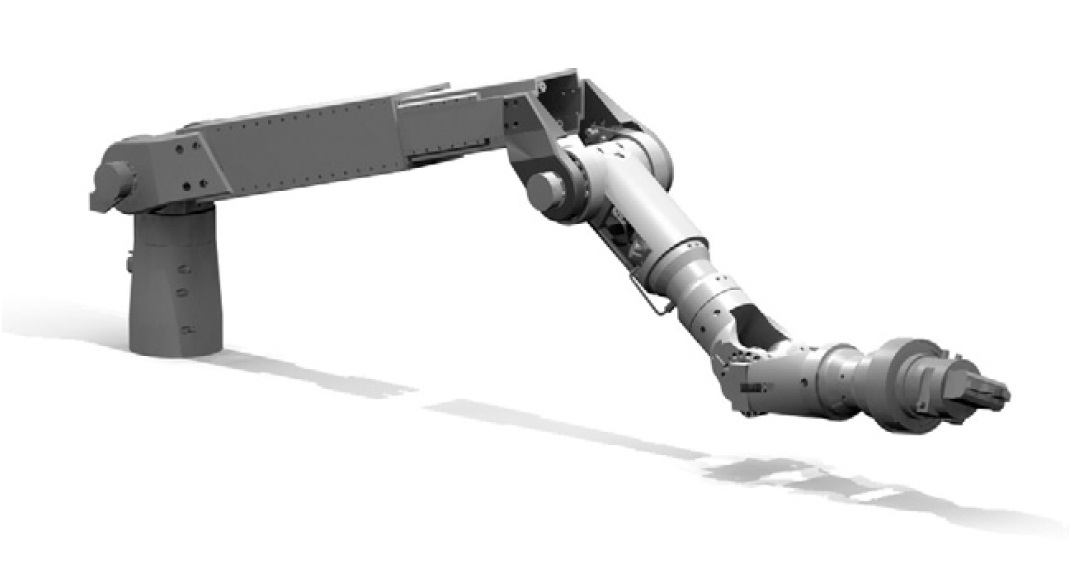
\includegraphics[width=0.7\textwidth]{FiguresSoA/WHMAN}
   \caption{Robot WHMAN de 6GDL.}
   \label{fig:WHMAN} 
\end{figure}

Tiene una capacidad de carga de 100 kg cuando esta totalmente extendido, en cuyo caso alcanza una distancia de 2.5 m medidos desde la articulación de la base. En la figura~\ref{fig:WHMAN} se muestra el diseño actual \cite{Nieminen2009}.
El WHMAN ha sido diseñado desde sus primeras fases para utilizar la potencia hidráulica del agua de acuerdo a los requisitos de ITER. Este manipulador es resistente a la radiación. Se estima que soporta una dosis de radiación de 300 Gy/h con una dosis acumulada de 1MGy. Debido a la elevada radiación, no utiliza electrónica digital, con lo cual, todos sus transductores est\'an basados en tecnología analógica.

%\subsection*{Robots MRI}
%Cabe mencionar que el reducida cantidad de máquinas superconductoras dará lugar a graves problemas logísticos cuando se quiera probar un robot completo bajo tales limitaciones.
%
%En pocas áreas, los robots se utilizan para posicionar objetos con precisión bajo la influencia de un alto campo magnético. Demuestra ser de interés para algunas intervenciones quirúrgicas. Es ahí donde aparecen los robots MRI. Un robot MRI es un robot médico capaz de operar dentro de una imagen de resonancia magnética (MRI), con el fin de realizar o ayudar en las intervenciones guiadas por imágenes (GII) \cite{Chinzei2001}.
%
%Hay pocos diseños para robots MRI, la mayoría de ellos trabajan lejos del campo magnético a fin de no sólo evitar la perturbación del dispositivo, sino también evitar la distorsión de la imagen como tal.
%En estos robots, tal como se presenta en \cite{Chinzei2001}, sólo las varillas largas pasivas de aleación de titanio o de material compuesto van en el campo magnético (\textless 0.5T).
%
%\begin{figure}[htbp]
%   \centering
%   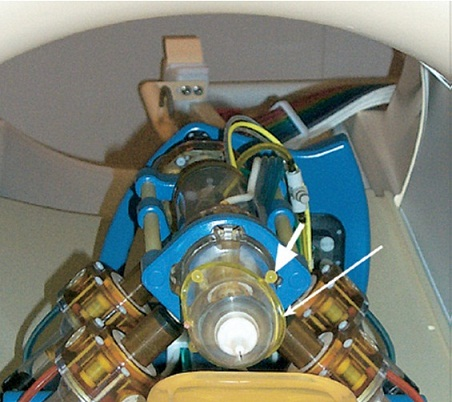
\includegraphics[width=0.5\textwidth]{FiguresSoA/MRI}
%   \caption{Robot MRI de al Universidad John Hopkins}
%   \label{fig:MIR} 
%\end{figure}
%
%Sin embargo, un equipo de la universidad John Hopkins ha sido diseñado un robot para funcionar con equipos de resonancias magnéticas \cite {Muntener2006}.
%Se dice que es el primer robot totalmente compatible con MRI y que cuenta con pruebas de compatibilidad de hasta 7T \cite{Muntener2006}.
%Dicho robot ha sido fabricado completamente con materiales paramagnéticos que evitan la distorsión del campo.
%Se basa en motores especiales, neumáticos, paso a paso y encoders ópticos con el fin de realizar movimientos precisos. Esto le permite manejar valores de precisión del orden de la fracción de milímetro. Es importante tener en cuenta que lo único que se le exige es ser compatible con resonancias magnéticas.



%\section{Telerobotica}
%Telepresence refers to a set of technologies which allow a person to feel as if they were present, to give the appearance of being present, or to have an effect, via telerobotics, at a place other than their true location.

%Telepresence requires that the users' senses be provided with such stimuli as to give the feeling of being in that other location. Additionally, users may be given the ability to affect the remote location. In this case, the user's position, movements, actions, voice, etc. may be sensed, transmitted and duplicated in the remote location to bring about this effect. Therefore information may be traveling in both directions between the user and the remote location.

%A popular application is found in telepresence videoconferencing, the highest possible level of videotelephony. Telepresence via video deploys greater technical sophistication and improved fidelity of both sight and sound than in traditional videoconferencing. Technical advancements in mobile collaboration have also extended the capabilities of videoconferencing beyond the boardroom for use with hand-held mobile devices, enabling collaboration independent of location.

%In a pioneering paper, Marvin Minsky attributed the development of the idea of telepresence to science fiction author Robert A. Heinlein: "My first vision of a remote-controlled economy came from Robert A. Heinlein's prophetic 1948 [sic] novel, Waldo," wrote Minsky. In his science fiction short story "Waldo" (1942), Heinlein first proposed a primitive telepresence master-slave manipulator system.

%The Brother Assassin, written by Fred Saberhagen in 1969, introduced the complete concept for a telepresence master-slave humanoid system. In the novel, the concept is described as follows: "And a moment later it seemed to all his senses that he had been transported from the master down into the body of the slave-unit standing beneath it on the floor. As the control of its movements passed over to him, the slave started gradually to lean to one side, and he moved its foot to maintain balance as naturally as he moved his own. Tilting back his head, he could look up through the slave's eyes to see the master-unit, with himself inside, maintaining the same attitude on its complex suspension."

%The term telepresence was coined in a 1980 article by the U.S. cognitive scientist Marvin Minsky, who outlined his vision for an adapted version of the older concept of teleoperation that focused on giving a remote participant a feeling of actually being present at a different location.[1]

%The first commercially successful telepresence company, Teleport (which was later renamed TeleSuite), was founded in 1993 by David Allen and Herold Williams.[2] Before TeleSuite, they ran a resort business from which the original concept emerged, because they often found businesspeople would have to cut their stays short to participate in important meetings. Their idea was to develop a technology that would allow businesspeople to attend their meetings without leaving the resorts so that they could lengthen their hotel stays.
%A Tandberg E20 high resolution videoconferencing phone meant to replace conventional desktop phones

%Hilton Hotels had originally licensed to install them in their hotels throughout the United States and other countries, but use was low. The idea lost momentum, with Hilton eventually backing out. TeleSuite later began to focus less on the hospitality industry and more on business-oriented telepresence systems. Shareholders eventually held enough stock to replace the company's original leadership, which ultimately led to its collapse.[citation needed] David Allen purchased all of the assets of TeleSuite and appointed Scott Allen as president, and Brian Kinne as EVP of the new company called Destiny Conferencing.

%Destiny Conferencing licensed its patent portfolio to HP which became the first large company to join the telepresence industry, soon followed by others such as Cisco and Polycom.[3] After forming a distribution agreement with Pleasanton-based Polycom, Destiny Conferencing sold on January 5, 2007 to Polycom for \$60 million.

%An important research project in telepresence began in 1990. Located at the University of Toronto, the Ontario Telepresence Project (OTP) was an interdisciplinary effort involving social sciences and engineering. Its final report stated that it "...was a three year, \$4.8 million pre-competitive research project whose mandate was to design and field trial advanced media space systems in a variety of workplaces in order to gain insights into key sociological and engineering issues. The OTP, which ended in December 1994, was part of the International Telepresence Project which linked Ontario researchers to their counterparts in four European nations. The Project’s major sponsor was the Province of Ontario, through two of its Centres of Excellence—the Information Technology Research Centre (ITRC) and the Telecommunications Research Institute of Ontario (TRIO)." [4]






